\documentclass{bioinfo}
%!TEX TS-program = pdflatex                                                    %
%!TEX encoding = UTF8                                                          %
%!TEX spellcheck = en-US                                                       %
%------------------------------------------------------------------------------%
% to compile use "latexmk --pdf main.tex"                                      %
%------------------------------------------------------------------------------%
% to count words 
% "pdftotext main_nofigs_nocaptions.pdf - | egrep -e '\w\w\w+' | iconv -f ISO-8859-15 -t UTF-8 | wc -w"
% -----------------------------------------------------------------------------%

\usepackage{url}
\usepackage[english]{babel}
\usepackage[utf8]{inputenc}
\usepackage[T1]{fontenc}
%\usepackage[pdftex]{graphicx} 
%\usepackage{graphics}
%\usepackage{hyperref}
\usepackage{float}
\floatplacement{figure}{H}
\usepackage{booktabs}     % nice tables
\usepackage{tabularx}     % even nicer tabular environments 
\usepackage{amsmath}
\usepackage{amsfonts}
\usepackage{amssymb}
%\usepackage{multicol}
\usepackage{listings}
\usepackage{tikz,times}
\usepackage{courier}
\usepackage[scaled]{beramono}

\usepackage{fancyvrb}

\usetikzlibrary{shapes,arrows}
\usetikzlibrary{arrows,positioning}
\usepackage{xcolor}
\usepackage[font=bf]{subfig}
\usepackage[inline]{trackchanges}

%%%%%%% setup track changes "editors"

\addeditor{mw}
\addeditor{lp}
\addeditor{psl}
\addeditor{ld}
\addeditor{sk}
\addeditor{vj}
\addeditor{jm}

%\usepackage{sectsty}
%\sectionfont{\normalsize\bfseries}
%\usepackage[labelfont=bf]{caption}
%\usepackage{endfloat} %place figures at end of document
%------------------------------------------------------------------------------%
%\captionsetup{
%%format = hang,                % caption format
%labelformat = simple,          % caption label : name and number
%labelsep = period,             % separation between label and text
%textformat = simple,           % caption text as it is
%justification = justified,     % caption text justified
%singlelinecheck = true,        % for single line caption text is centered
%font = {up,singlespacing},     % defines caption (label & text) font
%labelfont = {bf,footnotesize}, % NOTE: tiny size is not working
%textfont = footnotesize,
%%width = \textwidth,           % define width of the caption text
%skip = 1ex,                    % skip the space between float and caption
%listformat = simple,           % in the list of floats, label + caption
%}

%------------------------------------------------------------------------------%
%\hypersetup{
%    bookmarks=true,         % show bookmarks bar?
%    unicode=false,          % non-Latin characters in Acrobat’s bookmarks
%    pdftoolbar=true,        % show Acrobat’s toolbar?
%    pdfmenubar=true,        % show Acrobat’s menu?
%    pdffitwindow=false,     % window fit to page when opened
%    pdfstartview={FitH},    % fits the width of the page to the window
%    pdftitle={TheVirtualBain},    % title
%    pdfauthor={PSL},        % author
%    pdfsubject={ProposedArticle},   % subject of the document
%    pdfcreator={paupau},    % creator of the document
%    pdfnewwindow=true,      % links in new window
%    colorlinks=true,       % false: boxed links; true: colored links
%    linkcolor=red,          % color of internal links (change box color with linkbordercolor)
%    citecolor=blue,        % color of links to bibliography
%    filecolor=magenta,      % color of file links
%    urlcolor=blue           % color of external links
%}
%-----------------------------------------------------------------------
%\usepackage{subcaption}

%%%%%%%%%%%%%%%%%%%%%%%%%%%%%%%%%%%%%%%%%%%%%%%%%%%%%%%%%%%%%%%%%%%%%%%%%%%%%%%%
%%                             New and renew commands                         %%
%%%%%%%%%%%%%%%%%%%%%%%%%%%%%%%%%%%%%%%%%%%%%%%%%%%%%%%%%%%%%%%%%%%%%%%%%%%%%%%%
  
\renewcommand{\lstlistingname}{Code}
\renewcommand{\thesubfigure}{\Alph{subfigure}}
%\newcommand{\inputTikZ}[2]{\scalebox{#1}{\input{#2}}}
\newcommand*{\h}{\hspace{5pt}}   % for indentation
\newcommand*{\hh}{\h\h}          % double indentation
\newcommand*{\tvbmodule}[1]{{\textsc{#1}}}          % scientific modules in "simulator"
\newcommand*{\tvbdatatype}[1]{\textbf{\emph{#1}}}   % datatypes in "datatypes"
\newcommand*{\tvbclass}[1]{{\ttfamily\emph{#1}}}    % classes either in simulator mods or datatypes
\newcommand*{\tvbmethod}[1]{{\textsf{#1}}}          % methods
\newcommand*{\tvbattribute}[1]{{\ttfamily{#1}}}     % attributes
\newcommand*{\tvbtrait}[1]{{\ttfamily{#1}}}         % traited types
\newcommand{\TVB}{\textit{TheVirtualBrain }}

\newcommand{\matlab}{MATLAB}

%%%%%%%%%%%%%%%%%%%%%%%%%%%%%%%%%%%%%%%%%%%%%%%%%%%%%%%%%%%%%%%%%%%%%%%%%%%%%%%%
%%                            Colors and graphics                             %%
%%%%%%%%%%%%%%%%%%%%%%%%%%%%%%%%%%%%%%%%%%%%%%%%%%%%%%%%%%%%%%%%%%%%%%%%%%%%%%%%
\definecolor{palegreen}{HTML}{DAFFDA}
\definecolor{lightgray}{rgb}{0.15,0.15,0.15}
\definecolor{orange}{HTML}{FF7300}
\DeclareGraphicsExtensions{.jpg,.pdf,.png,.tiff}%,.mps,.bmp
\graphicspath{{figures/}}
 
%##--------------------------------------------------------------------------##%
%##                               START HERE                                 ##%
%##--------------------------------------------------------------------------##%
\copyrightyear{}
\pubyear{}

\begin{document}
\lstset{language=Python,
	captionpos=b,
	keepspaces=true,
	numbers=none,
	showspaces=false,
    float=*,
	basicstyle=\fontsize{8pt}{8}\ttfamily
	} 

\firstpage{1}

%%  Authorship and Title
\title[TVB]{Integrating neuroinformatics tools in TheVirtualBrain}
\author[Woodman {et~al}]{
        M. Marmaduke Woodman\,$^{1,*}$,  
        Laurent Pezard\,$^{1}$,  
        Lia Domide\,$^{3}$, 
        Stuart Knock\,$^{1}$, 
        Paula Sanz Leon\,$^{1}$, 
        Jochen Mersmann\,$^{2}$,
        Anthony R. McIntosh \,$^{4}$ and  
        Viktor Jirsa\,$^{1}$\footnote{to whom correspondence should be addressed: marmaduke.woodman@univ-amu.fr,
        viktor.jirsa@univ-amu.fr}}

\address{$^{1}$ \texttt{NEED CORRECT AFFILIATION FOR AIX-MARSEILLE UNIVERSITY, Marseille, France.}\\
         $^{3}$ Codemart, 13, Petofi Sandor, 400610, Cluj-Napoca, Romania.\\
         $^{2}$ CodeBox GmbH, Hugo Eckener Str. 7, 70184 Stuttgart, Germany.\\
         $^{4}$ Rotman Research Institute at Baycrest, Toronto, M6A 2E1, Ontario, Canada\\
        }

\history{}

\editor{}

\maketitle

%##--------------------------------------------------------------------------##%
%##                               ABSTRACT                                   ##%
%##--------------------------------------------------------------------------##%


\begin{abstract}
\section{}

TheVirtualBrain (TVB) is a neuroinformatics Python package representing the
convergence of clinical, systems, and theoretical neuroscience in the
analysis, visualization and modeling of neural and neuroimaging dynamics.
TVB is composed of a flexible simulator for neural dynamics measured across
scales from local populations to large-scale dynamics measured by
electroencephalography (EEG), magnetoencephalography
(MEG) and functional magnetic resonance imaging (fMRI), and 
core analytic and visualization functions,
 all accessible through a web browser user interface.
A datatype system modeling neuroscientific data ties together these pieces with
persistent data storage, based on a combination of SQL \& HDF5.
 These datatypes combine with adapters
allowing TVB to integrate other algorithms or computational systems.
TVB provides infrastructure for multiple projects and
multiple users, possibly participating under multiple roles. For example, a
clinician might import patient data to identify several potential lesion points
in the patient's connectome. 
A modeler, working on the same project, tests these points
for viability through whole brain simulation, based on the 
patient's connectome, and subsequent analysis of dynamical features.
TVB also drives research forward: the
simulator itself represents the culmination of several 
simulation frameworks in the modeling literature on human resting state. The 
availability of the numerical methods, set of neural mass models and 
forward solutions allows for the construction of a wide range of 
brain-scale simulation scenarios.
This paper briefly outlines the history and motivation for TVB, describing the 
framework and simulator, giving usage examples in the web UI
and Python scripting.
  
\section{Keywords:} large-scale brain network, simulation, web platform, Python,
connectivity, connectome, neural mass, time delays, functional MRI, 
electroencephalography, magnetoencephalography

\end{abstract}

%\tableofcontents

\section{Introduction}

%The neurosciences, and more generally, brain and behavioral sciences, imply
%extensive interactions among disciplines to advance our 
%appreciation for the relation between brain and behavior. 
%\footnote{The Human Brain Project one such example.} 
%The inherent challenge, however, lies in bringing together the distributed competences
%of many individuals or even institutions and exchanging across interdisciplinary
%borders using common techniques.  
%This situation is excerbated by the technical sophistication of modern
%data analysis and brain simulation, which often impedes their adoption 
%in the communtiy.
%
Neuroscience has evolved through extensive interactions among disciplines
to advance our appreciation of the relation between brain and behavior.
The interdisciplinary nature of the field presents formidable challenges
for effective collaboration.

These challenges call for two kinds of solutions. First, there is a need
for comprehensive, modern computational libraries written in widely
used and available programming languages; current examples include MNE-Python \citep{mnepython},
a Python package for treating M/EEG data via time-frequency analyses and inverse
solutions and the Brain Connectivity
Toolbox \citep{rubinov2010complex} for analyzing the graph theoretic
properties of structural and functional connectivity. Second, there is
a need for the implementation
of collaborative infrastructure for sharing not only data, but expertise; 
CARMEN \citep{austin2011carmen} and G-Node \citep{herz2008g} are two such
examples of developing platforms for collaborative work and data sharing, 
in the domains of cellular and systems neurophysiology.

TheVirtualBrain (TVB) provides new tools to facilitate the collaboration
between experimentalists and modelers by exposing both a comprehensive
simulator for brain dynamics and an integrative framework for the management,
analysis simulation of structural and functional data in an accessible,
web-based interface. The choice of Python was made based on its wide use as the
high-level language in scientific programming, the unparalleled open-source
libraries and tools available, and strong software engineering culture.  This
choice was confirmed by the publication of the first issue of Python in
Neuroscience and has made it possible for the entirety of TVB from the
numerical algorithms to the web server to be written in Python.

\subsection{The framework}

 \begin{figure*}
        \centering
        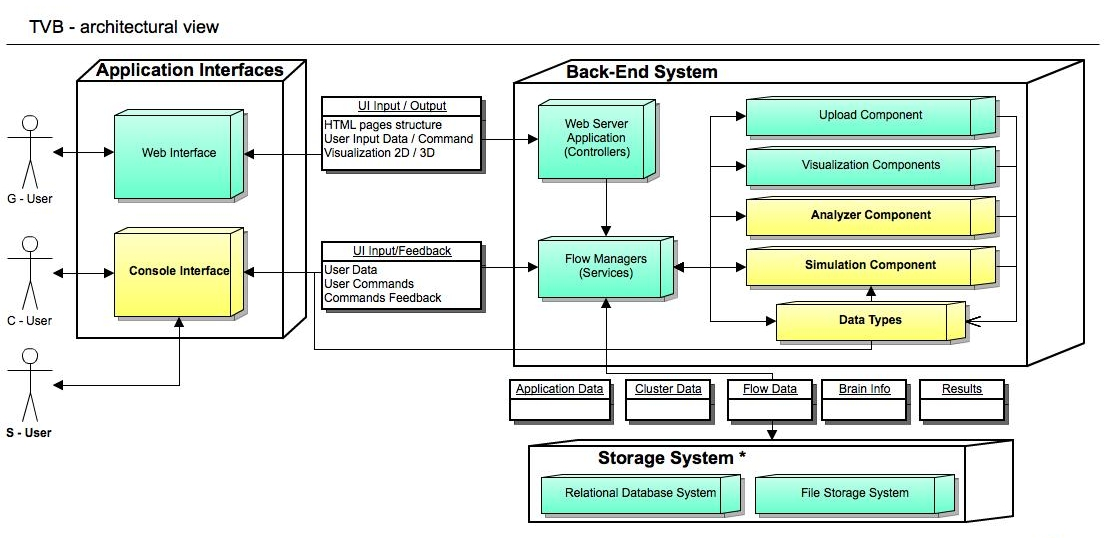
\includegraphics[width=0.90\textwidth]{images/architecture.jpg}
        \caption{TVB architecture: Yellow blocks are part of the scientific
            library of TVB, while the green blocks are part of TVB Framework.
            TVB provides two independent interfaces, depending on the
            interaction type desired the end-user (web or console).  TVB
            Storage layer is compulsory for the web interface, but it can be
	    switched on/off for the console interface.  The terms \textit{G-User},
	    \textit{C-User} and \textit{S-User} refer to users of the graphical,
	    console \& database and scripting components. Here, console interface
	    is conceptual and refers only to existing Python command lines, IPython
	    included. 
         }
        \label{fig:architecture}
 \end{figure*}

The TVB framework was developed to allow easy integration of any
computational tools along with a system for describing typical types of data.
Additionally, 
two main constraints for the framework were to provide a web
interface to allow remote collaboration and the
exchange of data (or simulation results) between users, especially for
users not comfortable programming. The web interface
and database backend are built on combination of 
the \textsf{CherryPy} and \textsf{SQLAlchemy} packages.
\footnote{The full list of dependencies can be found in the
project's documentation.}
The overall structure of TVB is depicted in Figure~\ref{fig:architecture}.

\subsection{The simulator}

A significant part of TVB is simulating large-scale brain networks. While
several existing simulators could have been adapted, we have estimated that
TVB style simulations are far enough outside the design of other simulators to
make a new development necessary. We discuss these reasons in the following. 

Existing neural network simulators typically focus either on abstract rate neurons, 
modelling  neurocognitive processes, or 
full multicompartmental neurons treating complex spatial
geometries, e.g. NEURON \citep{Hines_2001}, modelling the interaction of 
channel distributions in dendrites.  More recently, due to interest in
the computational properties of spiking neurons and their relevance to
experimental observations, simulators designed for spiking or oscillating neurons
have become prominent, including Brian \citep{Goodman_2009}, which we initially 
considered for our simulations.
In TVB the network is defined with neural mass or field
models \citep{Deco_2008a, Coombes_2010} rather than cellular models. The
spatial extent of the modeled dynamics is macroscopic and scales reasonably 
to the entire cortex, and uses empirical measurements of corticocortical
connectivity. Several technical issues are unique to this scale, such
as efficient handling of dense $N^2$ inter-regional delays and integration
of neural field-like models and connectivity on triangular meshes in 3D.
Finally, comparison with experimental data requires forward solutions
that transform physiological signals to the commonly
used imaging modalities such as EEG, MEG and fMRI need to be employed.
For these reasons, TVB required a new simulator, built around the paradigm
of whole-brain scale simulation.

\subsection{Obtaining and contributing to TVB}

The easiest way to get started with TVB is to download a distribution
from \url{http://www.thevirtualbrain.org}, which is available for Windows,
Mac OS X and Linux. This distribution includes
all of pieces, from the simulator to the web interface, and has no
requirements other than a modern web browser supporting WebGL, SVG and
HTML5.

Alternatively, because TVB is licensed under the GPL v. 2, the sources may be
readily obtained from the public Git repositories hosted on Github
\citep{dabbish2012social}, at 
\url{https://github.com/the-virtual-brain}. In order to use the simulator, 
only the standard scientific Python packages are required (NumPy \& SciPy).
The framework and web interface depend on a few more packages. 

We provide an API doc, built from the docs strings using Sphinx.
User's, Contributor's and Developer's manuals are also provided with TVB
distributions in PDF format. The source files (in .rst) are available
through the Github repository \url{https://github.com/the-virtual-brain/docs}.  
In addition, IPython notebooks \citep{PerezGranger_2007}
for interactive tutorials are provided. These are based on the
demonstration scripts provided with the scientific library, and
include a more detailed description of the scientific goal (if
applicable), the components and stages of a simulation as well as a
brief description in the case of reproducing previous work. Users
interacting with \TVB GUI may also benefit from these tutorials
(\url{https://github.com/the-virtual-
brain/scientific_library/wiki/Tutorials}) when displayed as snippets
with IPython nbviewer. 

Additionally, the user interface provides an online help overlay, that pulls
information from the User's manual.



\section{Architecture}

TVB is logically and technically divided into a scientific
library and a framework package, where the scientific library includes
datatypes, basic analyses and the simulator, while the
framework handles execution infrastructure, the web-based user interface and
data storage.  The scientific library can function as an independent Python
module, but the framework depends the scientific library for datatype definitions
and algorithms. 

\subsection{Basic Concepts}

The TVB framework is oriented around data and the operations that introduce,
generate, transform and visualize the data. The relevant interface classes
derive from the metaclasses in Python's abstract base class library, and
provide a foundation for defining any type of data from a tuple to a
set of EEG channel labels to a simulation, each of which is defined by a class
implemented the datatype interface and possessing one or more datatypes as 
attributes. An operation is the execution of any algorithm that
has been \emph{adapted} to the framework in a class implementing the abstract
adapter interface, and range from the simulator to data importers to
visualizers.  The goal of these twin, generic abstractions is to provide a
solid basis on which to implement a storage back-end, workflow management and a
number of features to support collaborative work. 

Importantly, the framework supports both the use of the web-based graphical
interface and the console interface for advanced user and developers. Where
the console user does not wish to rely on the database persistence, this 
storage layer can be disabled. Specifically, TVB uses the notion of \emph{profile} to 
identify in what context the application is currently running,
and thus what components are expected to be loaded.
For example, when the scientific library is used alone, a specific profile (\emph{library profile}) class 
gets linked as current profile, which, in this case, disables data storage and the web interface. Other profiles available
in TVB are: \emph{command profile}, \emph{deployment profile} (with web interface), and \emph{test profiles}.

\subsection{Datatypes and storage}

\subsubsection{TVB Traits}

Because an explicit goal of TVB is to provide a user interface to each of the
entities and algorithms contained within, it is necessary at some point to
provide metadata on how to built that interface. A traits system was
developed, similar to that of IPython or EPD, allowing for
attributes on a TVB class to be written out with its full metadata. An extensive
set of building blocks implements from numeric types and arrays to
lists, tuples, string, and dictionaries.

\begin{center}
	\begin{table*}[ht]

	\begin{tabularx}{\textwidth}{lll}
      		\toprule
      		Traited Attribute    & Description  \\ 
      		\midrule
		default 	& Default value for current attribute. Will be set on any new instance if not specified otherwise in the constructor.  \\
		console\_default & Define how a default value can be computed for current attribute, when console interface is enabled. \\
		range	& Specify the set of accepted values for current attribute. Mark that this attribute is usable for parameter space exploration. \\

		label		& Short text to be displayed in UI, in front of current attribute. \\
		doc		& Longer description for current attribute. To be displayed in UI as help-text. \\
		required	& Mark current attribute as required for when building a new instance of the parent class. \\
		locked	& When present and \emph{True}, current attribute will be displayed as read-only in the web interface. \\

		options	& Used for attributes of type \emph{Enumerate}, specifying the accepted options as a list of strings. \\
		filters\_ui	& SQL filters on other attributes, to be applied in UI. \\
		select\_multiple & When \emph{True}, current attribute will be displayed as a select with multiple options in UI (default is single-select) \\
		order	& Optional number identifying the index at which current attribute will be displayed in UI. \\
				& When negative, the attribute is not displayed at all. Ascending order for indices is considered when displaying. \\

		use\_storage	& When \emph{False}, current attribute is not stored in database or file storage. \\
		file\_storage	& Valid values for this attribute are: \emph{None} , \emph{HDF5}, or  \emph{expandable\_HDF5}, \\
					& When \emph{None}, current attribute is not stored in the file-storage at all. When \emph{HDF5}, we use regular HDF5 file storage. \\
					& When \emph{expandable\_HDF5} value is set, a HDF5 stored in chunks is used. \\
		\bottomrule
    	\end{tabularx}
  	\caption{TVB currently available Traited Attributes}
  	\label{tab:traits}
	\end{table*}
\end{center}


When methods of such a class with annotated attributes are invoked, they may use
the traited attributes directly, accessing either a default value or one given
during the instantiation of the object. Additionally, this allows the web-based
user interface to introspect a class for all of its attributes and their
descriptions, to provide help and choose the proper display form. The explicit
typing also allows such classes to be nearly automatically mapped to storage
tables, providing persistence, when the storage layer is enabled.  Lastly,
because such metadata is used to build the docstring of a class, the console
user also may obtain extensive descriptions of class, attributes, methods and
arguments in the usual way. Table \ref{tab:traits} lists the various parts 
of a traited attribute and how they are used. 


\subsubsection{Datatypes}

To allow for the handling of various kinds of data within the TVB framework, 
the \textit{Datatype} abstraction considers a class with several 
attributes to fully describe (expected type, short label, long
description, order in UI, required or not, etc.) the entity. 

In TVB, datatypes represent the common language, to be used between different
application parts: like uploaders, analyzers, simulator and visualizers.
Some of the algorithms are producing these datatypes, while others are reading
them as input.  In order to decouple the definition and several usages of such
entities, datatypes are declared outside the algorithms and shared between them.
For example an instance of datatype TimeSeriesRegion is created by the
Simulator, and it can be accepted as input for several visualizers or analyzed
by principal component analysis and cross coherence algorithms.

Technically, TVB datatypes are annotated Python classes, which
contain one or more fields and associated descriptive information, as
well as methods for operating on the data they contain. The definition of a
datatype is achieved using TVB's traiting system, mentioned in previous section.

For example, the \texttt{Connectivity} datatype, which may elsewhere
be represented by a simple $N$ by $N$ NumPy array, is written as a class
in which one of the attributes, \texttt{weights}, is a explicitly typed 
\texttt{FloatArray}, and the declaration of this type is complemented by
explicit label, default values, and documentation strings. See
Code~\ref{lst:ConnectivityData}.

\begin{lstlisting}[caption={The ConnectivityData listing},
                   label={lst:ConnectivityData}]
class ConnectivityData(MappedType):

  region_labels = arrays.StringArray( 
	label="Region labels", 
        doc="""Labels for the regions ...""")

  weights = arrays.FloatArray( 
	label="Connection strengths",
        doc="""... strength of connections ...""")

  tract_lengths = arrays.FloatArray( 
	label="Tract lengths",
        doc="""... length of myelinated fibre tracts.""")

   speed = arrays.FloatArray( 
	label="Conduction speed", 
	default=numpy.array([3.0]), 
	file_storage=core.FILE_STORAGE_NONE,
         doc="""... matrix of conduction speeds ...""")

  centres = arrays.PositionArray( 
	label="Region centres",
        doc="""... locations for the region centers""")
\end{lstlisting}
	

\subsection{Adapters}

The framework expects algorithms to be adapted by providing a class
that inherits from the base adapter, \texttt{ABCAdapter}, implementing 
the adapter interface:

\begin{lstlisting}[caption={Excerpt of the ABCAdapter},
                   label={lst:ABCAdapter}]
class AdapterExample(ABCAdapter):

  @abstractmethod
  def get_input_tree(self):
  	pass

  def configure(self, **kwargs):
  	pass

  @abstractmethod
  def launch(self):
  	pass
\end{lstlisting}

\noindent where \texttt{get\_input\_tree} builds a dictionary of input
arguments required for the algorithm and for
presenting menus and fields in the user interface, \texttt{configure} allows the 
adapter to initialize itself and its algorithm based on arbitrary arguments
and \texttt{launch} invokes the algorithm.
Additional methods include \texttt{get\_output}, \texttt{get\_required\_memory\_size},
and
\texttt{get\_required\_disk\_size}.

TVB employs adaptors for data creation, upload, simulation, analysis, visualization
and export. 

Note that the adapters and datatypes are intended to provide full 
power and flexibility of the framework; when the simulator is invoked from
the web-based UI, it is done so through a \texttt{SimulatorAdapter} which,
despite being relatively complex, is built with \emph{traits} all the way down.

It is reasonable to ask what such a scheme offers over the more 
conventional approach of Python, where presumably it would have been
sufficient that each adapter consist of a class with an \texttt{\_\_init\_\_}
and \texttt{\_\_call\_\_} method, in the case of a function type. 
We note that because in the case of TVB, the context in which an object
is used is more varied, e.g. not simply initialized but loaded through 
SQLAlchemy's object relational mapping, and that the adapter is required to perform more tasks
than just initialization and invocation, e.g. provide expected shape of 
result, estimate occupied memory and do not start if insufficient resources are found on current machine,
 it was advantageous to create a distinct set of interfaces built on top of
the abstract base class framework provided by Python's standard library.

\paragraph{An adapter for FastICA}

An example of an adapter applying the FastICA algorithm to each of the 
state variables in a simulation time series is given in Code \ref{lst:ica}.

\begin{lstlisting}[language=Python]
class ICAAdapter(ABCAsynchronous):
    
    _ui_name = "Independent Component Analysis"
    _ui_description = "ICA for a TimeSeries input DataType."
    _ui_subsection = "ica"
    
    
    def get_input_tree(self):
        algorithm = fastICA()
        algorithm.trait.bound = self.INTERFACE_ATTRIBUTES_ONLY
        tree = algorithm.interface[self.INTERFACE_ATTRIBUTES]
        filt = FilterChain(fields=
                [FilterChain.datatype + '._nr_dimensions'],
                operations=["=="], values=[4])
        for node in tree:
            if node['name'] == 'time_series':
                node['conditions'] = filt
        return tree
    
    
    def get_output(self):
        return [IndependentComponents]
    
    def configure(self, time_series, n_components=None):
        self.input_shape = time_series.read_data_shape()
        log_debug_array(LOG, time_series, "time_series")
        
        self.algorithm = fastICA()
        self.algorithm.n_components = \
                n_components or self.input_shape[2]
        
    def get_required_memory_size(self, **kwargs):
        used_shape = (self.input_shape[0], 1, 
                self.input_shape[2], self.input_shape[3])
	input_size = numpy.prod(used_shape) * numpy.float64().itemsize
        output_size = self.algorithm.\
                            result_size(used_shape)
        return input_size + output_size  
    
    def launch(self, time_series, n_components=None):
        ica_result = IndependentComponents(
            source=time_series,
            n_components=int(self.algorithm.n_components),
            storage_path=self.storage_path)
        
        # 4-D simulation time series
        node_slice = [slice(self.input_shape[0]), 
                None, slice(self.input_shape[2]), 
                slice(self.input_shape[3])]
        
        ts = TimeSeries(use_storage=False)
        for var in range(self.input_shape[1]):
            node_slice[1] = slice(var, var + 1)
            ts.data = time_series.read_data_slice(
                    tuple(node_slice))
            self.algorithm.time_series = ts 
            partial_ica = self.algorithm.evaluate()
            ica_result.write_data_slice(partial_ica)
        ica_result.close_file()
        return ica_result
\end{lstlisting}

\paragraph{Interfacing with MATLAB}

One of the well-known libraries for characterizing anatomical 
and functional connectivity is the \emph{Brain Connectivity Toolbox} 
\citep{Rubinov_2010}. 
Because it is written in MATLAB, with developers who prefer MATLAB, we 
chose not to port routines of the library to Python but instead build
a MATLAB adapter that runs arbitrary MATLAB code. 

This generic Matlab adapter works by generating at runtime a script with MATLAB code, 
wrapping the script call in Python with a try-except clause,  
loading and saving the workspace before and after the call,
generating a workspace \texttt{.mat} file, invoking the MATLAB or Octave
executable, and loading the resulting workspace file. 

Despite invocation of MATLAB being a relatively slow operation, this works
without problems in a single user situation, and where Octave is available, it
is quite fast. In the case that many operations are necessary, they can be
batched into the same run.

\section{Simulator}

The simulator in TVB resembles popular neural network simulators in 
many fundamental ways, both mathematically and in terms of informatics 
structures, however we have found it necessary to introduce auxiliary
concepts particularly useful in the modeling of large scale brain 
networks. In the following, we will highlight some of the interesting
principles and capabilities of TVB's simulator and give rough characterization
of the execution time and memory required in typical simulations.

\subsection{Node dynamics}

	In TVB, nodes are not considered to be abstract neurons nor necessarily
	small groups thereof, but rather large populations of neurons. Concretely,
	the main assumption of the neural mass modeling approach in TVB is that
	large pools of neurons on the millimeter scale are strongly approximated
	by population level equations describing the major statistical modes of
	neural dynamics \citep{Freeman_1975book}. Such an approach is certainly not
	new; one of the early examples of this approach consist of the well known
	Wilson-Cowan equations \citep{Wilson_1973}. Nevertheless, there are
	important differences in the assumptions and goals from modeling of
	individual neurons, where the goal may be to reproduce correct spike
	timing or predict the effect of  a specific neurotransmitter. A second
	difference lies in coupling: chemical coupling is often assumed to be
	pulsatile, or discrete, between neurons, whereas for mesoscopic models it is considered
	continuous. Typically the goal of neural mass modeling is to study the
	dynamics that emerge from the interaction of two or more neural masses and
	the network conditions required for stability of a particular
	spatiotemporal pattern. In the following, we shall  briefly discuss some
	of the models available in TVB.

	This modeling paradigm may be contrasted with ensemble models modelling
	the dynamics of large populations of neurons with a certain state space
	(\cite{de1993stochastical, omurtag2000simulation, knight2000dynamics, gerstner2000population};
	see \cite{Deco_2008a} for a review).
	The large number of neurons impart the state
	space with a probability density, and population density methods describe the
	evolution of this density via the Fokker-Planck (FP) equation \citep{risken1996fokker}
	comprised of flow and dispersion terms.  This approach assumes
	that the afferents on neurons in one population are uncorrelated.
	Neural mass models, from this paradigm, are obtained as a special case
	when the full ensemble density dynamics is replaced by a mass at one
	point in state space and its dynamics summarize the movement of density
	in state space, losing information on the changes in shape of the
	density.  In the full, nonlinear FP form, different density moments can
	couple, even within and between populations, meaning the membrane
	potential variance of one population could affect the average of
	another. Neural mass models ignore this possibility by coupling only
	the first moments, though this may be overcome by e.g. extending mass
	models with more than one mode 
	\citep{Stefanescu_2008, Stefanescu_2011}. 
	TVB does not implement density methods via the FP
	equation because the additional moments required to derive
	physiologically relevant variables (such as LFP or firing rate), would
	add an additional level of complexity.  

	In TVB, many neural mass models from the literature are available, including
	the often used Jansen-Rit model of rhythms and evoked responses arising from
	coupled cortical column \citep{Zetterberg_1978, Jansen_1995,Spiegler_2010}. 
	\citeauthor{David_2003}'s slightly modified form has been extensively
	applied within a Bayesian framework known as Dynamic Causal Modeling (DCM) 
	for modeling neuroimaging data via estimation of biophysical parameters of 
	underlying network models \citep{David_2003, friston2003dynamic, david2006dynamic}.
	The Jansen-Rit model is a biophysical one, whose state variables and parameters 
	are readily interpretable with respect to experiments, however it has
	at least six state equations involving several exponential expressions. For
	cases where it is desirable to have a simpler and more performant 
	model, a generic two-dimensional oscillator model is also provided by TVB 
        \citep{strogatz2001nonlinear, guckenheimer1983nonlinear}.
	This model produces damped, spike-like or sinusoidal oscillations, which, in
	the context of a network, permit the study of network phenomena, such as 
	synchronization of rhythms or propagation of evoked potentials.
	Other models implemented in TVB include the Wilson-Cowan description of
	functional dynamics of neural tissue \citep{Wilson_1972}, the Kuramoto
	model describing synchronization \citep{Kuramoto_1975, Cabral_2011}, two
	and three dimensional statistical mode-level models describing populations with
	excitability distributions \citep{Stefanescu_2011, Stefanescu_2008}, a
	reduction of \citeauthor{Wong_2006}'s (\citeyear{Wong_2006}) model as presented 
	by \cite{Deco_2013} and a lumped version of Liley's model \citep{Liley_1999, Steyn-Ross_1999}.
	Lastly, adding a model only requires subclassing a base \texttt{Model} class and
	providing a  \texttt{dfun} method to compute the right hand sides of the
	differential equations. 

\subsection{Network structure}

	The network of neural masses in TVB simulations directly follows from  two
	 geometrical constraints on cortical dynamics. The first is the
	large-scale white matter fibers that form a non-local and heterogeneous
	(translation variant) connectivity, either measured by anatomical tracing
	(CoCoMac, \cite{Koetter_2004}) or diffusion-weighted imaging 
    \citep{Hagmann_2008, Honey_2009, Bastiani_2012}.
    The second is that of horizontal projections
	along the surface, which are often modeled with a translation invariant
    connectivity kernel, approximating a neural field (however, as with other
    parameters in the simulator, connectivity kernel parameters that vary 
	across space can also be used).

	TVB does not assume that the network structure is constant during the
	simulation, but does not currently implement the modeling of structural
	modulation. This can however be added by hand during simulation.

	\subsubsection{Large-scale connectivity}

	The large-scale region level connectivity at the scale of centimeters,
	resembles more a traditional neural network than a neural field, in that,
	neural space is discrete,  each node corresponding to a neuroanatomical
	region of interest, such as V1, etc. It is at this level that inter-regional 
	time delays play a large role, whereas the time delays due to 
	lateral, local projections are subsumed under the dynamics of the node.

	It is often seen in the literature that the inter-node coupling functions
	\textit{are} part of the node model itself. In TVB, we have instead 
	chosen to factor such models into the intrinsic neural mass dynamics, where each 
	neural mass's equations specify how connectivity contributes to the
	node dynamics, and the coupling function, which specifies how the activity
	from each region is mapped through the connectivity matrix. Common coupling 
	functions are provided such as the linear, difference and periodic functions
	often used in the literature.

	\subsubsection{Local connectivity}

	The local connectivity of the cortex at the scale of millimeters provides
	a continuous 2D surface along horizontal projections connect 
	cortical columns. Such a structure has previously been modeled by
	neural fields \citep{Amari_1977, Jirsa_1997, Liley_1999}. In TVB, a cortical mesh, 
	as obtained from structural MRI data and simplified, provides a spatial 
	discretization on which neural masses are placed and connected with a
	local connectivity kernel, itself only a function of the geodesic distance
	between the two masses. This is considered to provide a reasonable
	approximation of a neural field, the appropriateness of which depends on the properties
	of the mesh and the imaging modalities that sample the activity simulated
	on the mesh \citep{Spiegler_2013}. In fact,
	the implementation of the local connectivity kernel is such
	that is can be re-purposed as a discrete Laplace-Beltrami operator,
	allowing for the implementation of true neural field models that 
	use a second-order spatial derivative as their explicit spatial term.

	TVB currently provides several connectivity kernels, of which a Gaussian
	is one commonly used. Once a cortical surface mesh 
	and connectivity kernel and its parameters are chosen, the geodesic
	distance (i.e. the distance along the cortical surface) is evaluated
	between all neural masses \citep{Mitchell1987}, and a cutoff is chosen
	past which the kernel falls to 0. This results in a sparse matrix that 
	is used during integration to implement the approximate neural field. 

\subsection{Integration of stochastic delay differential equations}

	In order to obtain numerical approximations of the network model 
	described above, TVB provides both deterministic and stochastic
	Euler and Heun integrators,
	following standard numerical solutions to stochastic
	differential equations \citep{Kloeden_1995,Mannella_2002,Mannella_1989}.

	While the literature on numerical treatment of delayed or 
	stochastic systems exists, it is less well known how to treat 
	the presence of both. For the moment, the methods implemented by TVB
	treat stochastic integration separately from delays. 
	This separation coincides with a modeling assumption that in
	TVB the dynamical phenomena to be studied are largely determined
	by the interaction of the network structure and neural mass dynamics, 
	and that stochastic fluctuations do not fundamentally reorganize the
	solutions of the system \citep{Ghosh_2008,Deco_2009,Deco_2011,Deco_Senden_2012}.

	Due to such a separation, the implementation of delays in the
	regional coupling is performed outside the integration step,
	by indexing a circular buffer containing the recent simulation 
	history, and providing a matrix of delayed state data to the 
	network of neural masses. While the number of pairwise
	connections rises with $n_{region}^2$, where $n_{region}$ is
	the number of regions in the large-scale connectivity, 
	a single buffer is used, with a shape
	$(horizon, n_{cvar}, n_{region})$ where $horizon = max(delay) + 1$,
	and
	$n_{cvar}$ is the number of coupling variables. Such a scheme helps 
	lower the memory requirements of integrating the delay equations.

\subsection{Forward solutions}

	TVB provides forward solutions to generate neuroimaging data from 
	simulated neural activity based on biophysical models 
	\citep{Buxton_2004, Jirsa_2002}. Practically, it is also often
	necessary to simply reduce the size of data, especially in the case of 
	surface simulations. TVB implements these two functionalities in
	a set of classes called \texttt{Monitors}, each of which receives
	the raw simulation output and applies a spatial, temporal or spatiotemporal
	kernel to the output to obtain the simulation output passed to the
	user or stored. 

	Where necessary, monitors employ more than one internal buffer. In the case of 
	the fMRI monitor, a typical sampling frequency of simulation may be upward of 
	64 kHz, and the haemodynamic response function may last several seconds, 
	using only a single buffer could require several gigabytes of memory for the 
	fMRI monitor alone. Given that 
	the time-scale of simulation and fMRI differ by several orders of magnitude, 
	the subsequent averaging and downsampling is justified. 

	In the cases of the EEG and MEG monitors, the temporal kernel implements a simple
	temporal average, and the spatial kernel consists of a so-called lead-field matrix as typically
	derived from a combination of structural imaging data, 
	providing the locations and orientations of the neural sources and the locations
	and orientations of the EEG electrodes and MEG gradiometers and magnetometers. 
	As the development and implementation of such lead-fields is well developed
	elsewhere \citep{Sarvas_1987,Hamalainen_1989,Jirsa_2002,Nolte2003,Gramfort_2010}, 
	TVB provides access to the well-known OpenMEEG package.

\subsection{Performance}

	A priority of the simulator in TVB is to attain a high level of performance
	while remaining in pure Python. In order to see where the simulator 
	spends most of its time, we have profiled 
	a set of eight characteristic simulations
	%on both memory use, specifically the heap size as measured by Valgrind's 
	%\texttt{massif} tool \citep{nethercote2007valgrind}, 
    	on function timing as measured by the 
	\texttt{cProfile} module of the standard library. 
	
	Measurements were
	performed on an HP Z420 workstation, with a single Xeon E5-1650
	six-core CPU running at 3.20 GHz, L1-3 cache sizes 384 KB, 1536 KB
	and 12 MB respectively, with main memory 4 x 4 GB DDR3 at 1600 Mhz,
	running Debian 7.0, with Linux kernel version 3.2.0-4-amd64. 
	The 64-bit Anaconda Python distribution was used with additional Accelerate
	package which provides acceleration of common routines based on the 
	Intel Math Kernel Library. A Git checkout of the trunk branch of TVB 
	was used with SHA \texttt{6c644ab3b5}.

	Eight different simulations were performed corresponding to the combinations of
	either the generic 2D oscillator or Jansen-Rit model, region-only
	or use of cortical surface, and two conduction speeds, $v_c = 2.0$ and
	$v_c = 20.0$ (m/s). In each case, a temporal average monitors at 512 Hz
	is used, and the results are discarded. The region-only simulation was
	run for one second while the surface simulation was run for 100 ms. 

		%% AUTO GENERATED DO NOT MODIFY

		%% round times to two digits, center on '.'
		\begin{table}
		{\footnotesize \begin{tabular}{r | r | l }
		Sim. &        Time (s) &                     Module/Function \\
		\hline \\
		R / G2D / 20  &         11.72 & \texttt{<numpy.core.multiarray.array>} \\
		&          6.14 & \texttt{numpy.lib.npyio}, \texttt{loadtxt} \\
		 &         5.18 & \texttt{tvb.simulator.simulator}, \texttt{\_\_call\_\_} \\
		 &         3.18 & \texttt{numpy.lib.npyio}, \texttt{pack\_items} \\
		 &          2.56 & \texttt{numexpr.necompiler}, \texttt{evaluate} \\
		\hline
		2 &         11.87 & \texttt{<numpy.core.multiarray.array>} \\
		&         6.10 & \texttt{numpy.lib.npyio}, \texttt{loadtxt} \\
		 &         5.54 & \texttt{tvb.simulator.simulator}, \texttt{\_\_call\_\_} \\
		 &         3.16 & \texttt{numpy.lib.npyio}, \texttt{pack\_items} \\
		 &         2.50 & \texttt{numexpr.necompiler}, \texttt{evaluate} \\
		\hline
		 JR / 20  &         14.21 & \texttt{<numpy.core.multiarray.array>} \\
		&         9.99 & \texttt{tvb.simulator.simulator}, \texttt{\_\_call\_\_} \\
		 &         7.28 & \texttt{tvb.simulator.models}, \texttt{dfun} \\
		 &           6.20 & \texttt{numpy.lib.npyio}, \texttt{loadtxt} \\
		 &         3.24 & \texttt{numpy.lib.npyio}, \texttt{pack\_items} \\
		\hline
		2 &         14.21& \texttt{<numpy.core.multiarray.array>} \\
		&         10.57& \texttt{tvb.simulator.simulator}, \texttt{\_\_call\_\_} \\
		 &         7.40& \texttt{tvb.simulator.models}, \texttt{dfun} \\
		 &         6.12& \texttt{numpy.lib.npyio}, \texttt{loadtxt} \\
		 &         3.25& \texttt{numpy.lib.npyio}, \texttt{pack\_items} \\
		\hline
		S / G2D / 20 &         126.61& \texttt{<\_csc.csc\_matvec>} \\
		&         57.56& \texttt{<numpy.core.multiarray.array>} \\
		 &         56.17& \texttt{<gdist.local\_gdist\_matrix>} \\
		 &           9.05& \texttt{<numpy.core.\_dotblas.dot>} \\
		 &         7.56& \texttt{numpy.lib.npyio}, \texttt{loadtxt} \\
		\hline
		2 &         125.95& \texttt{<\_csc.csc\_matvec>} \\
		&         57.75& \texttt{<numpy.core.multiarray.array>} \\
		 &         56.16& \texttt{<gdist.local\_gdist\_matrix>} \\
		 &         12.10& \texttt{<numpy.core.\_dotblas.dot>} \\
		 &         7.37& \texttt{numpy.lib.npyio}, \texttt{loadtxt} \\
		\hline
		JR / 20 &         126.31& \texttt{<numpy.core.multiarray.array>} \\
		&         56.37& \texttt{<gdist.local\_gdist\_matrix>} \\
		 &         19.52& \texttt{<numpy.core.\_dotblas.dot>} \\
		 &         9.47& \texttt{tvb.simulator.models}, \texttt{dfun} \\
		 &         8.87& \texttt{<mtrand.RandomState.normal>} \\
		\hline
		2 &         126.09& \texttt{<numpy.core.multiarray.array>} \\
		&         56.79& \texttt{<gdist.local\_gdist\_matrix>} \\
		 &          29.10& \texttt{<numpy.core.\_dotblas.dot>} \\
		 &         14.18& \texttt{<mtrand.RandomState.normal>} \\
		 &         9.57& \texttt{tvb.simulator.models}, \texttt{dfun} \\
		\hline

		\end{tabular}}
		\caption{Profiling results for several simulation types, ``R'' for region 
		level simulations, ``S'' for surface level. ``G2D'' signifies the generic
		two-dimensional oscillator whereas ``JR'' is the Jansen-Rit model. Finally,
		either 20 m/s or 2 m/s conduciton velocity was used. Time is given as the
		total time spent in the method or function listed in the right column.}
		\label{tab:profiling}
		\end{table}


	As can be seen in Table \ref{tab:profiling}, the time spent during simulation
	is dominated by numerical, built-in methods (marked by those functions surrounded by angle
	brackets) from the NumPy and SciPy libraries, with the exception of a few
	calls to the \texttt{loadtxt} function, which is necessary when importing TVB's
	datatypes the first time. For surface simulations, it is also necessary to compute
	a local distance matrix \texttt{<gdist.local\_gdist\_matrix>}. Nevertheless, 
	some of the time spent on array operations such as computing the right hand sides 
	of the differential equations can be 
	recovered by using the \texttt{numexpr} module which eliminates the 
	use of temporary arrays. 

\section{User Interaction}

\subsection{Graphical Interface Interaction}

		A graphical web interface was designed for user friendly
		interaction with TVB . The web interface is accessible locally or
		remotely through a web browser; it can be used by different types of
		users, including those without programming knowledge, and it offers
		good support while the user is learning TVB concepts and workflow
		expectations.  

		\subsubsection{Projects, Accounts, Operations \& Data}

		TVB uses several kinds of entities to model user actions
        and artifacts.

 \begin{figure}[!htbp]

		\centering
		\subfloat[][]{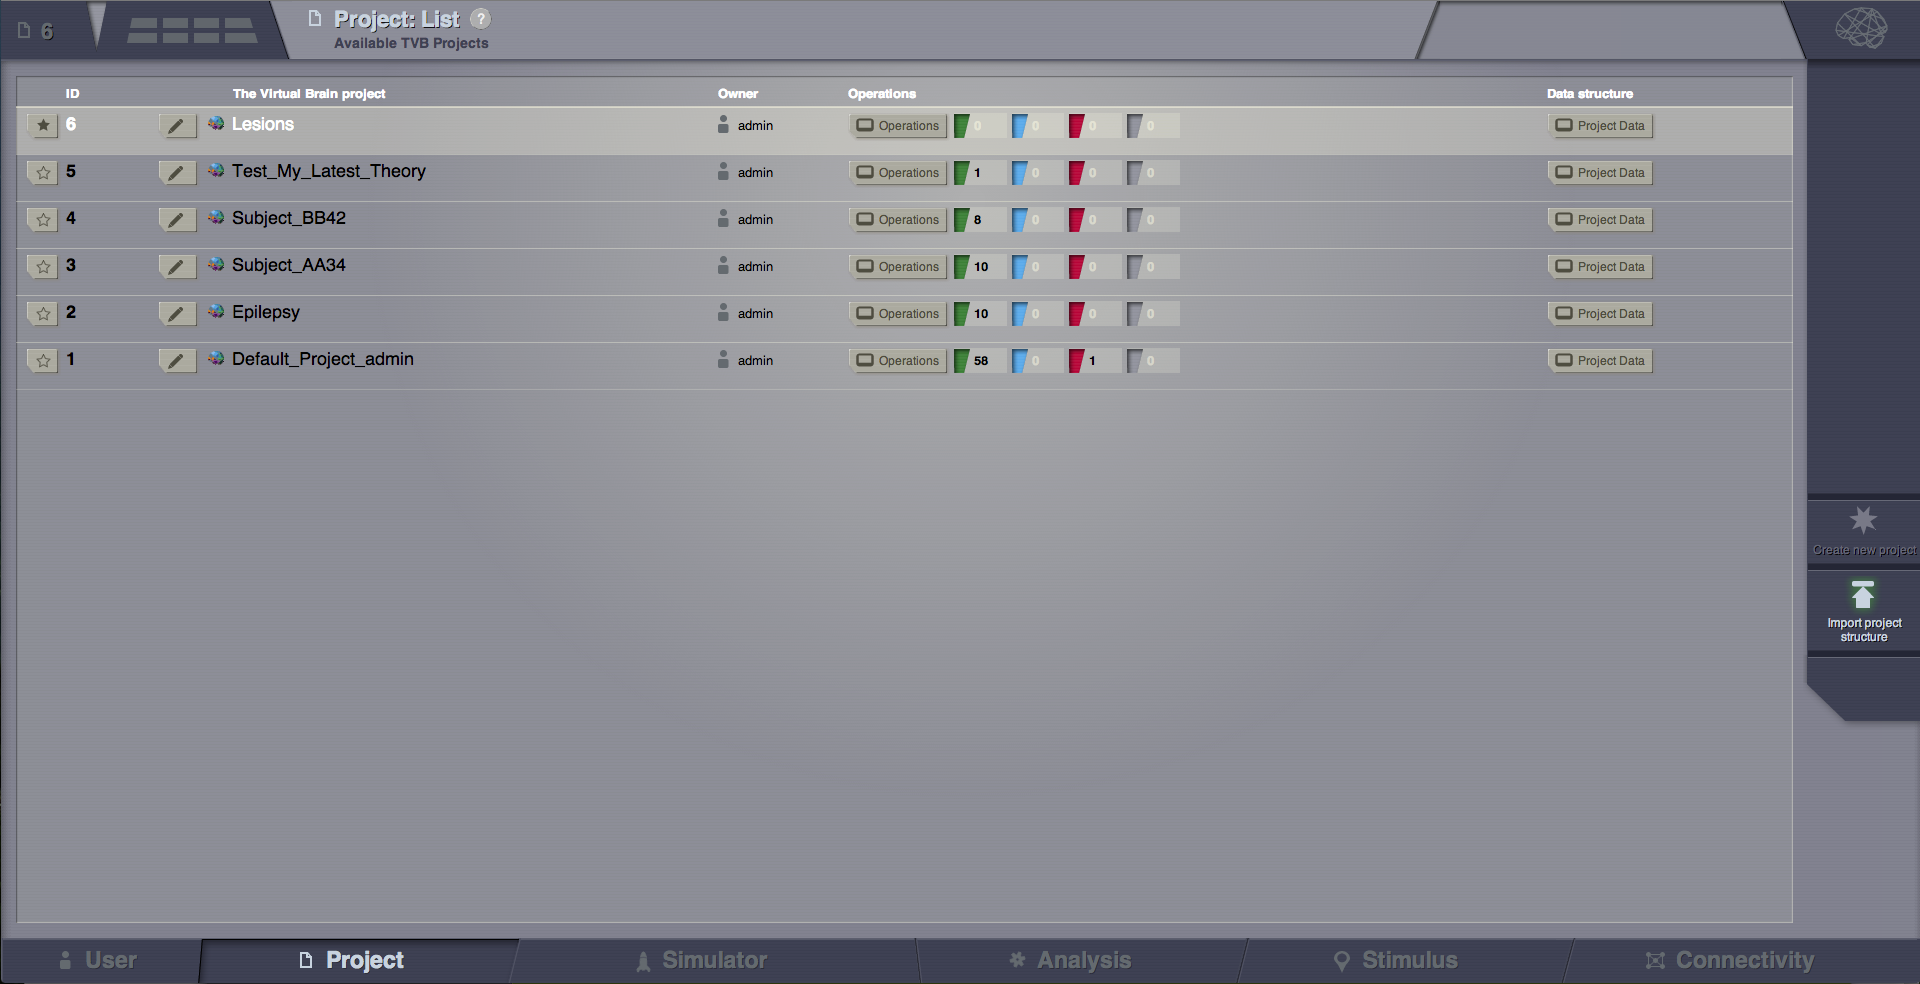
\includegraphics[width=0.47\textwidth]{images/ui_projects.png}}
		\\
		\subfloat[][]{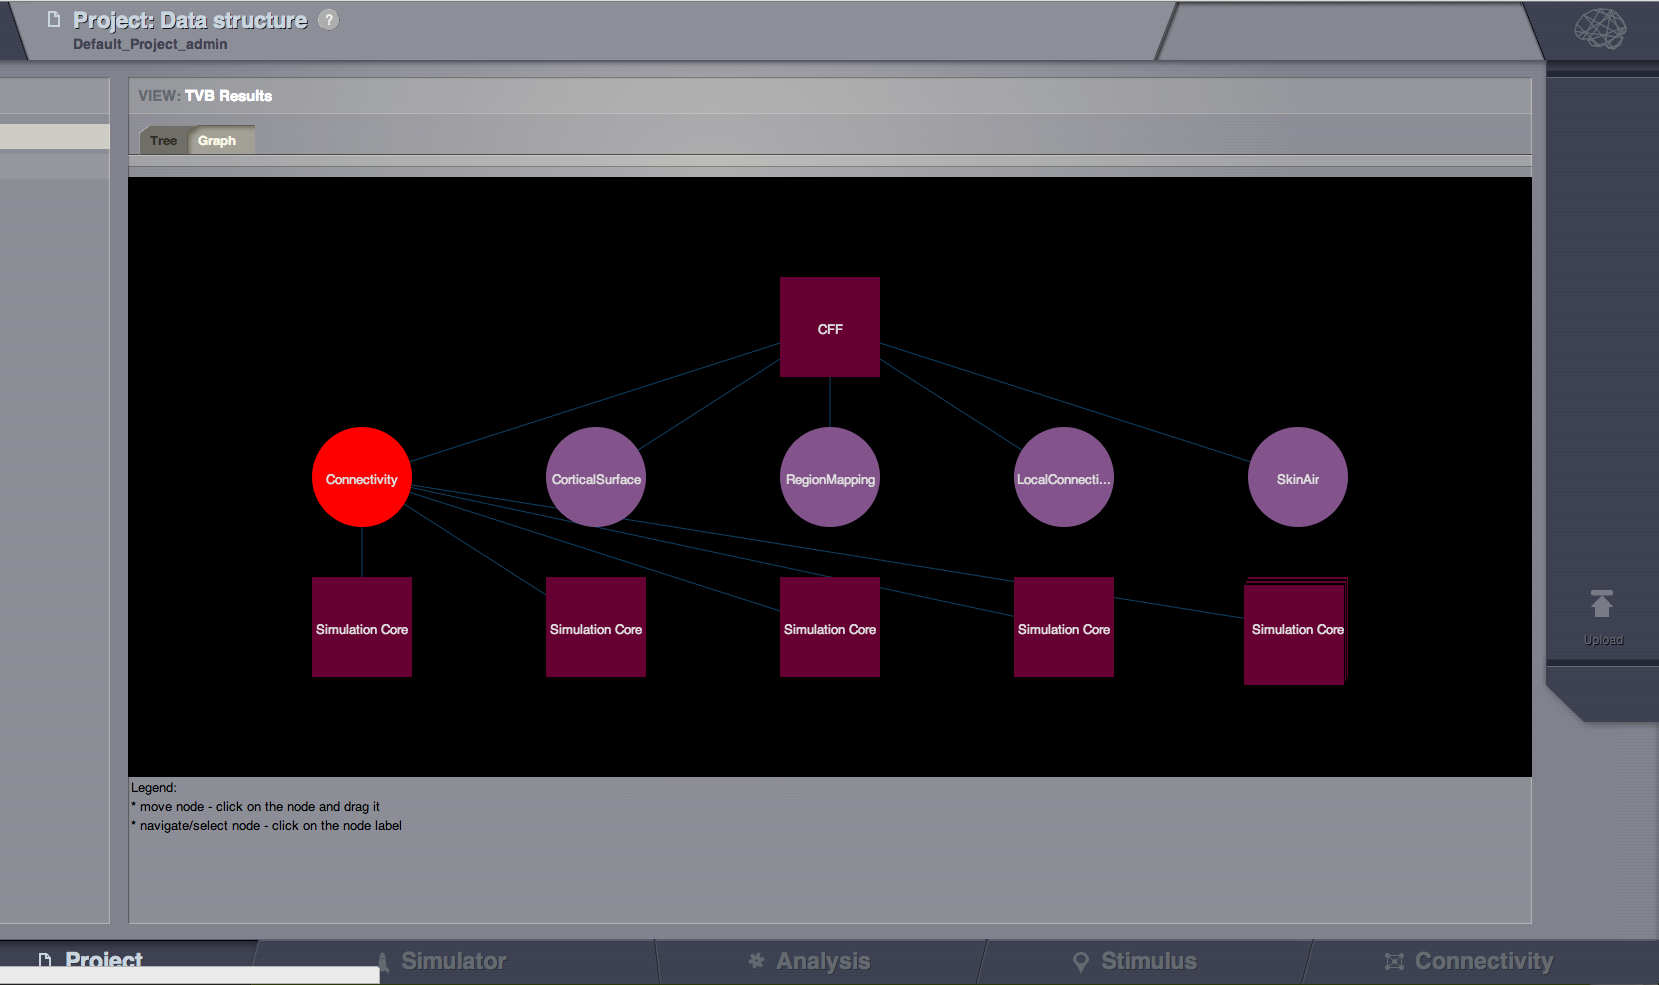
\includegraphics[width=0.47\textwidth]{images/ui_project_graph.png}}
		\\
		\subfloat[][]{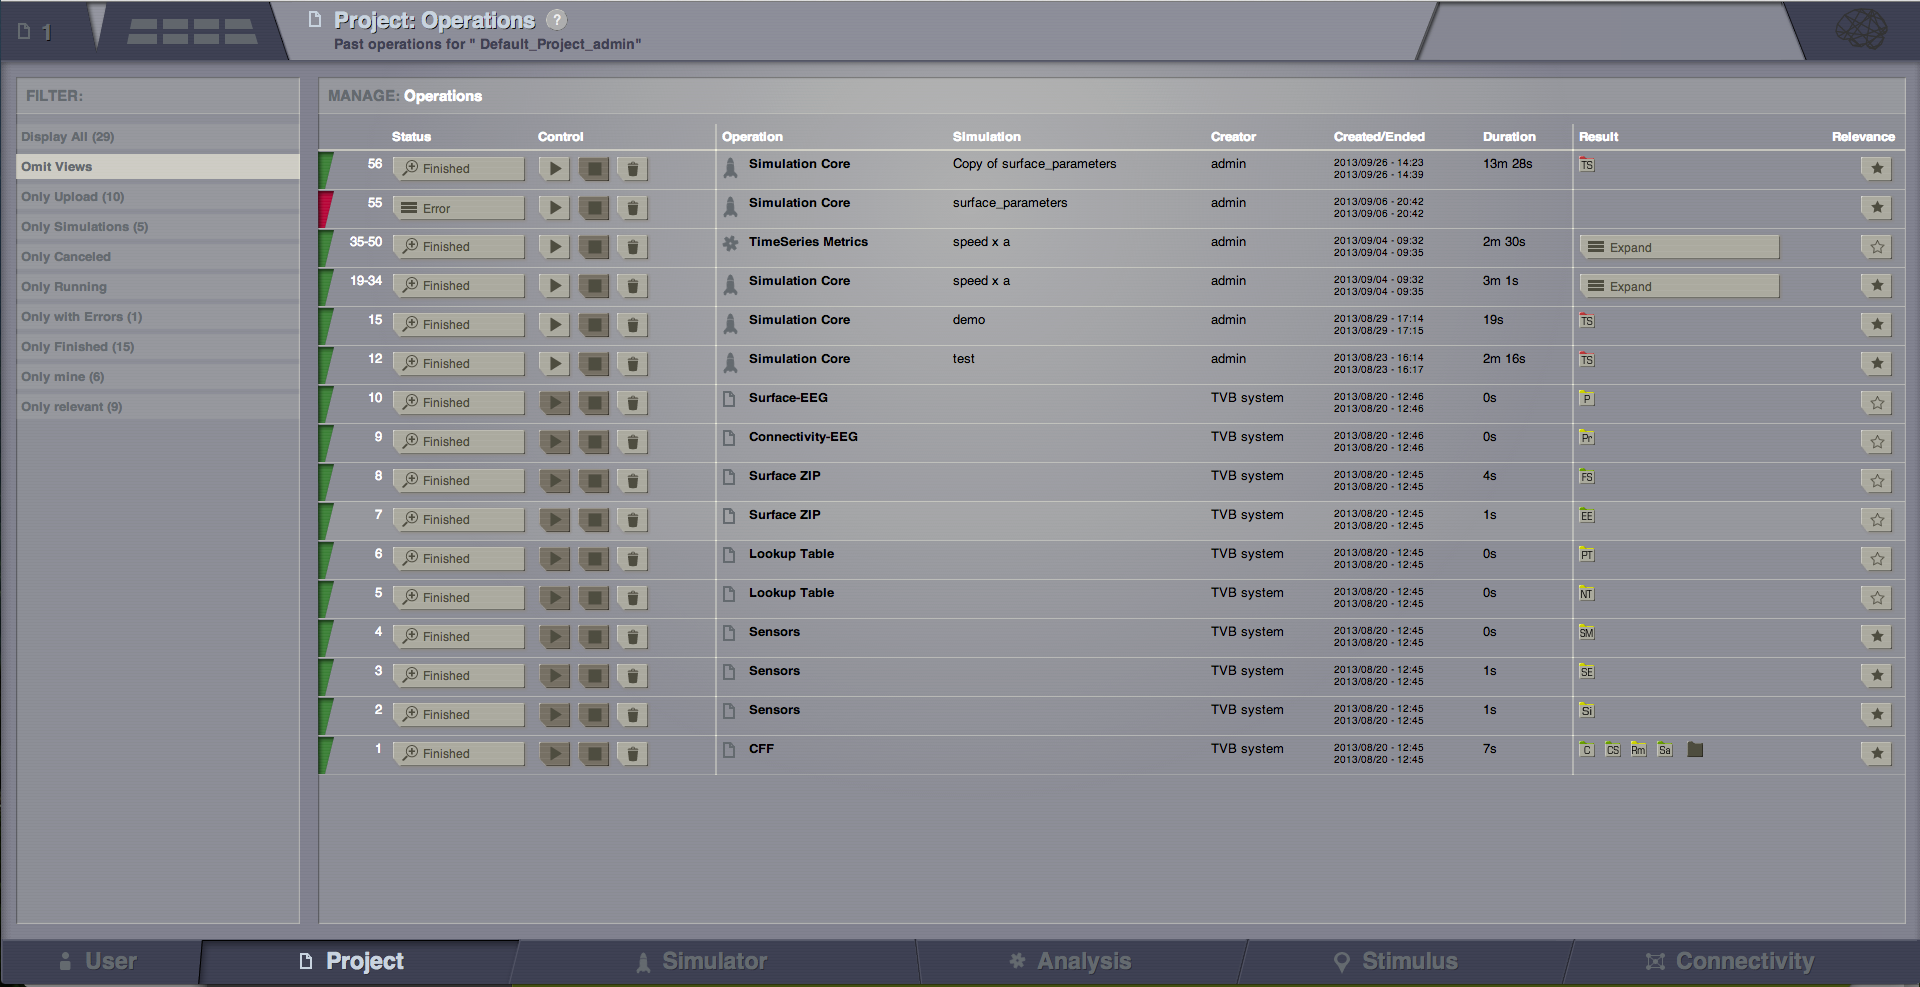
\includegraphics[width=0.47\textwidth]{images/ui_project_operations.png}}
		\\
		\subfloat[][]{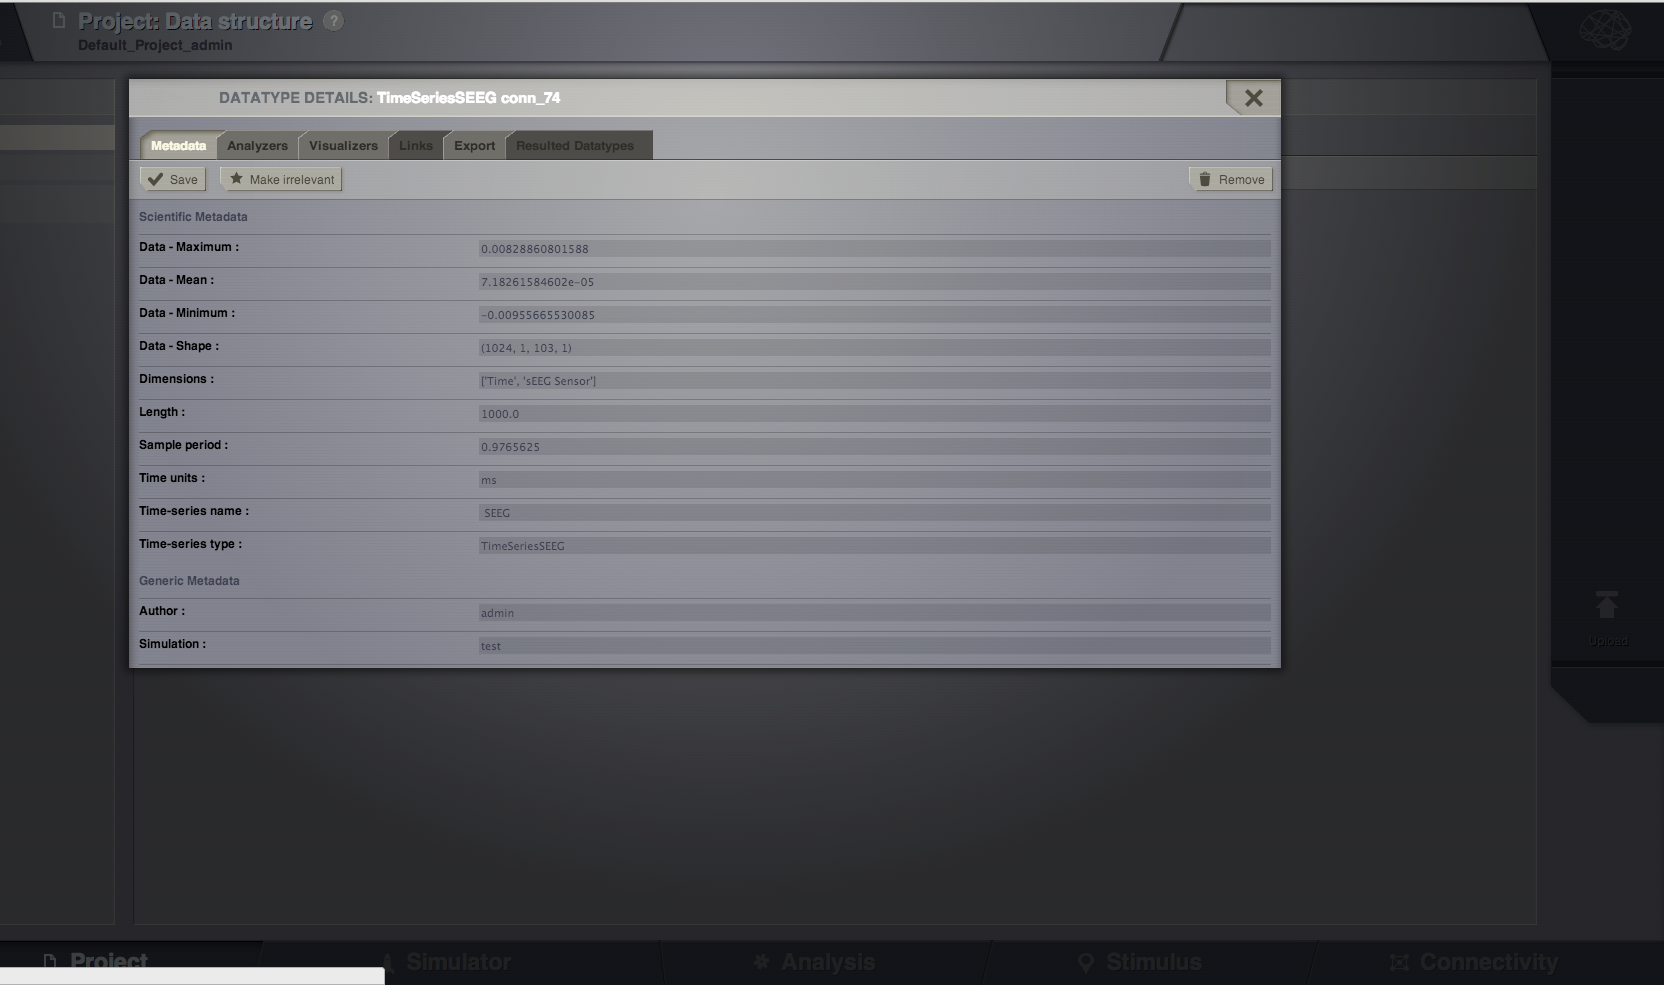
\includegraphics[width=0.47\textwidth]{images/ui_project_datatype_details.png}}
		\caption{\TVB data organization
		(A) View all projects
		(B) 2D graph display of operations with their input and output datatypes 
		(C) View all operations in current project with their status, duration, results, etc
		(D) Datatype details and further available operations for it. This menu becomes available after clicking a datatype result from several places in TVB }
				\label{fig:project}
\end{figure}

		An \emph{Account} or \emph{User} is needed for accessing TVB through
		the web interface.  When TVB web interface is started for the first
		time, the user is requested to provide a username and 
		password for the first account, which acts as an \emph{administrator}.
        Thereafter, others users on the same TVB server can \emph{register}
		for accounts, which are validated by the administrator account.

		A \emph{Project} in TVB is a logical grouping of data and operations: 
        for example, one could choose to
		create a project for each experiment in TVB, while others might
		create projects for each subject of a group. Each project has a single
		user (or account) as owner, but a project may be shared
		with other users to allow for collaboration.

		The execution of an adapter results in an operation, in the
		context of a project. For example, operations are created for each
		simulation, a spectral analysis or surface visualization. 
        Operations have show their status in the user interface, changing from
		\emph{started} to \emph{canceled}, \emph{finished successfully} or
		\emph{finished with error}. 

		A \emph{workflow} in TVB is, conceptually, sequence of operations from simulation,
        through analyses, to visualization(s). A particular workflow applies
		 a default \emph{tag} on the associated operations and
		datatypes.
        The user may also add custom tags to further organize data.

		\subsubsection{Simulator Interface}

		\begin{figure}[!htbp]

		\centering
			\subfloat[][]{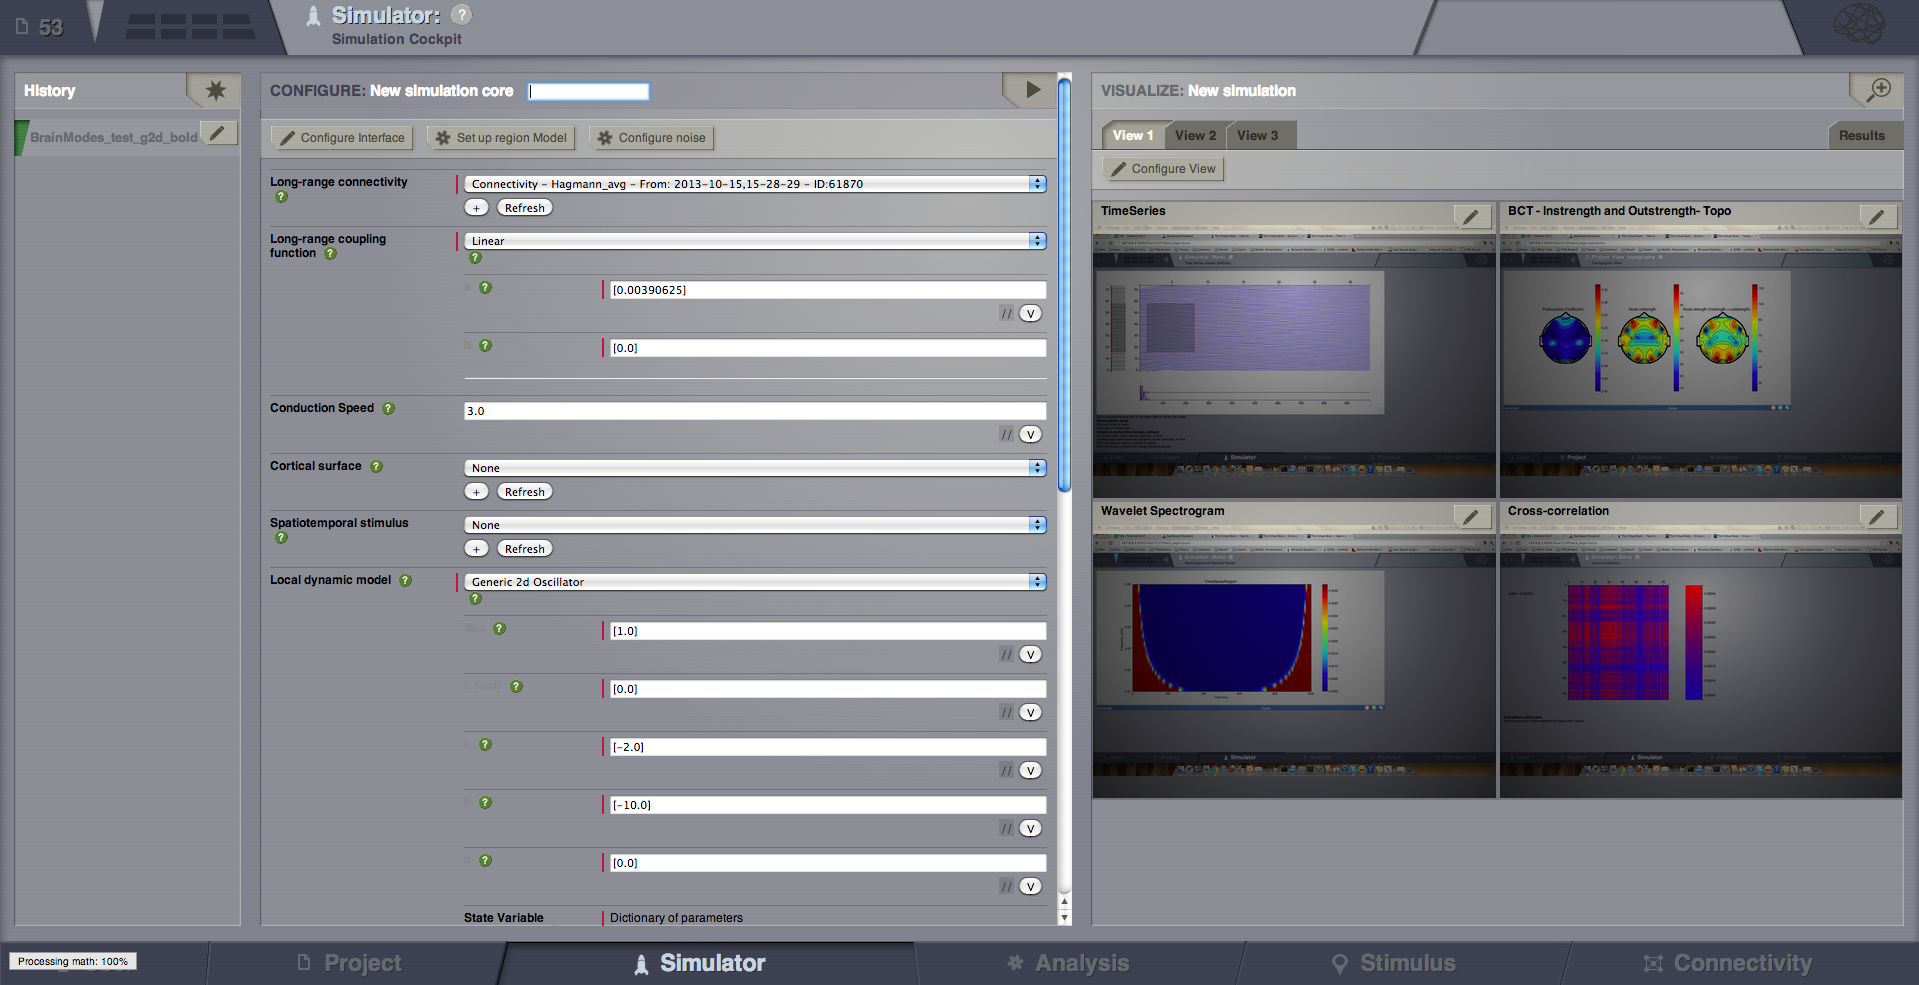
\includegraphics[width=0.47\textwidth]{images/ui_simulator.png}}
			\\
			\subfloat[][]{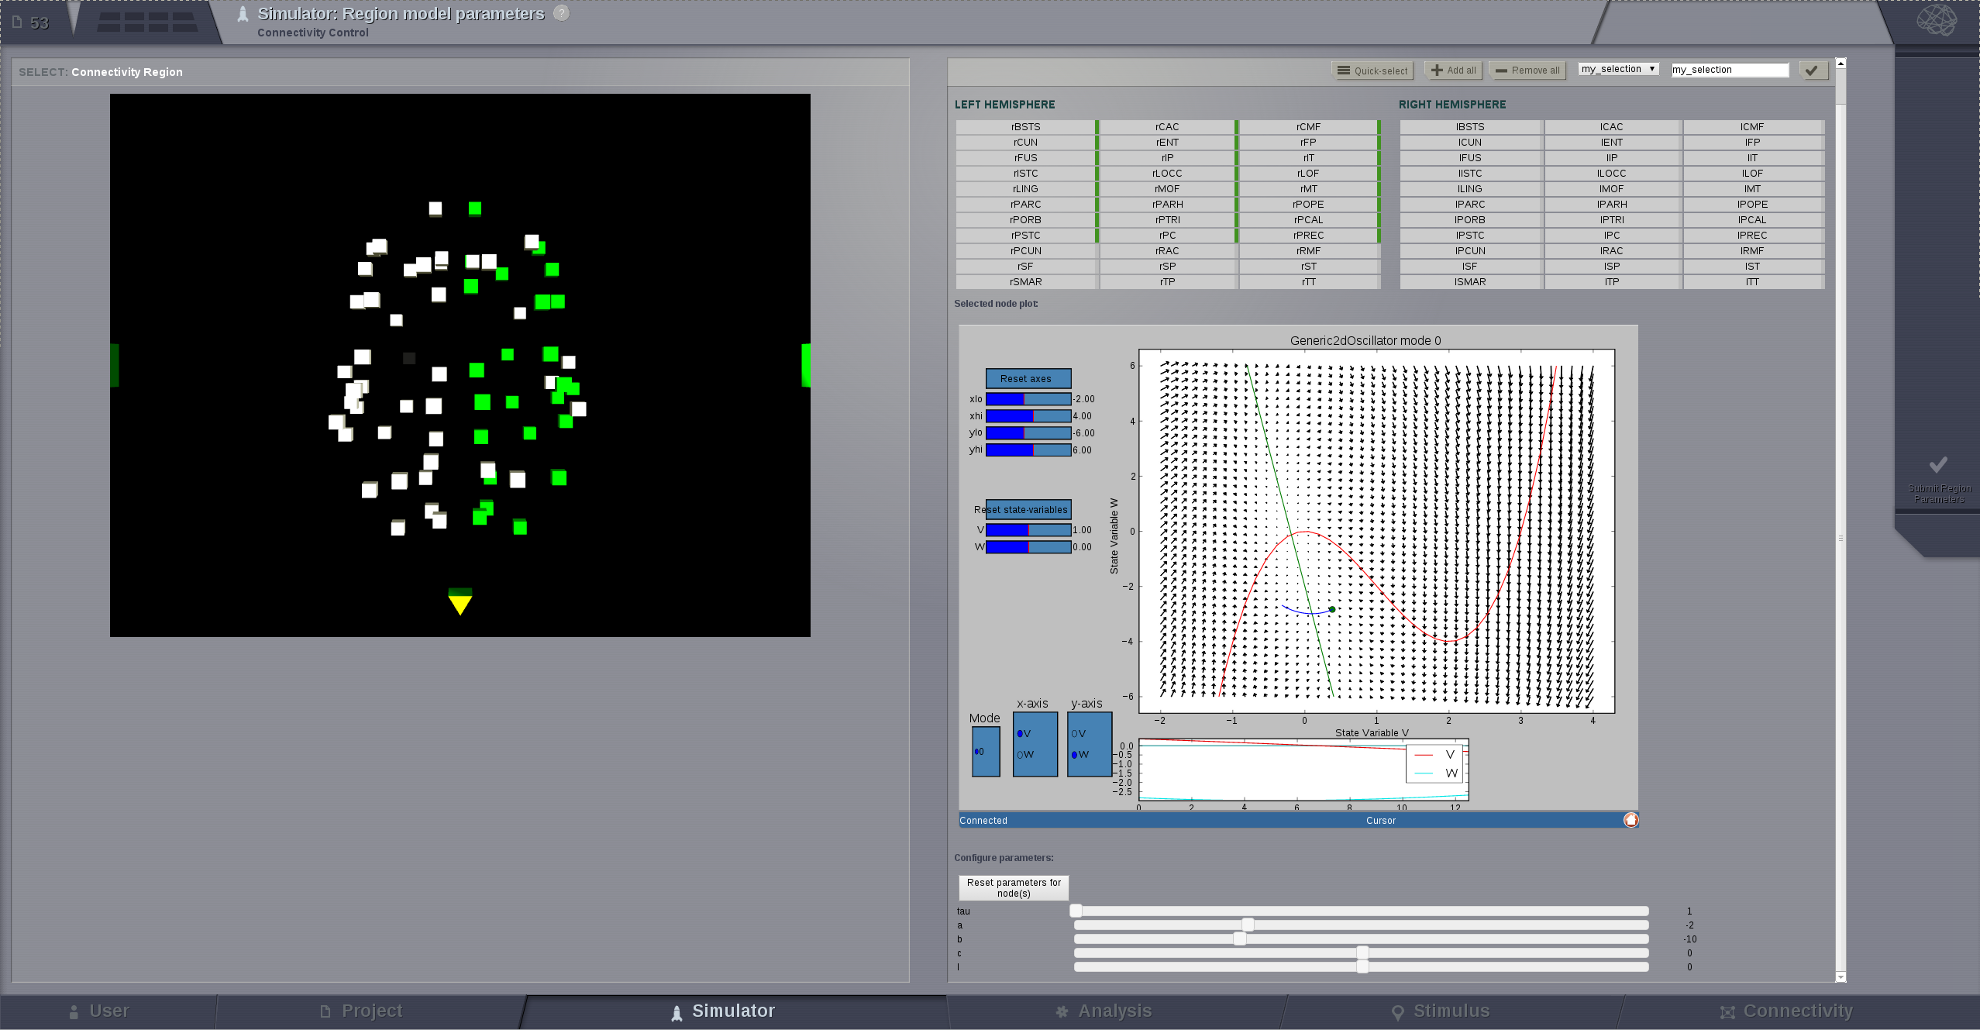
\includegraphics[width=0.47\textwidth]{images/ui_simulator_setup_region.png}}
			\\
			\subfloat[][]{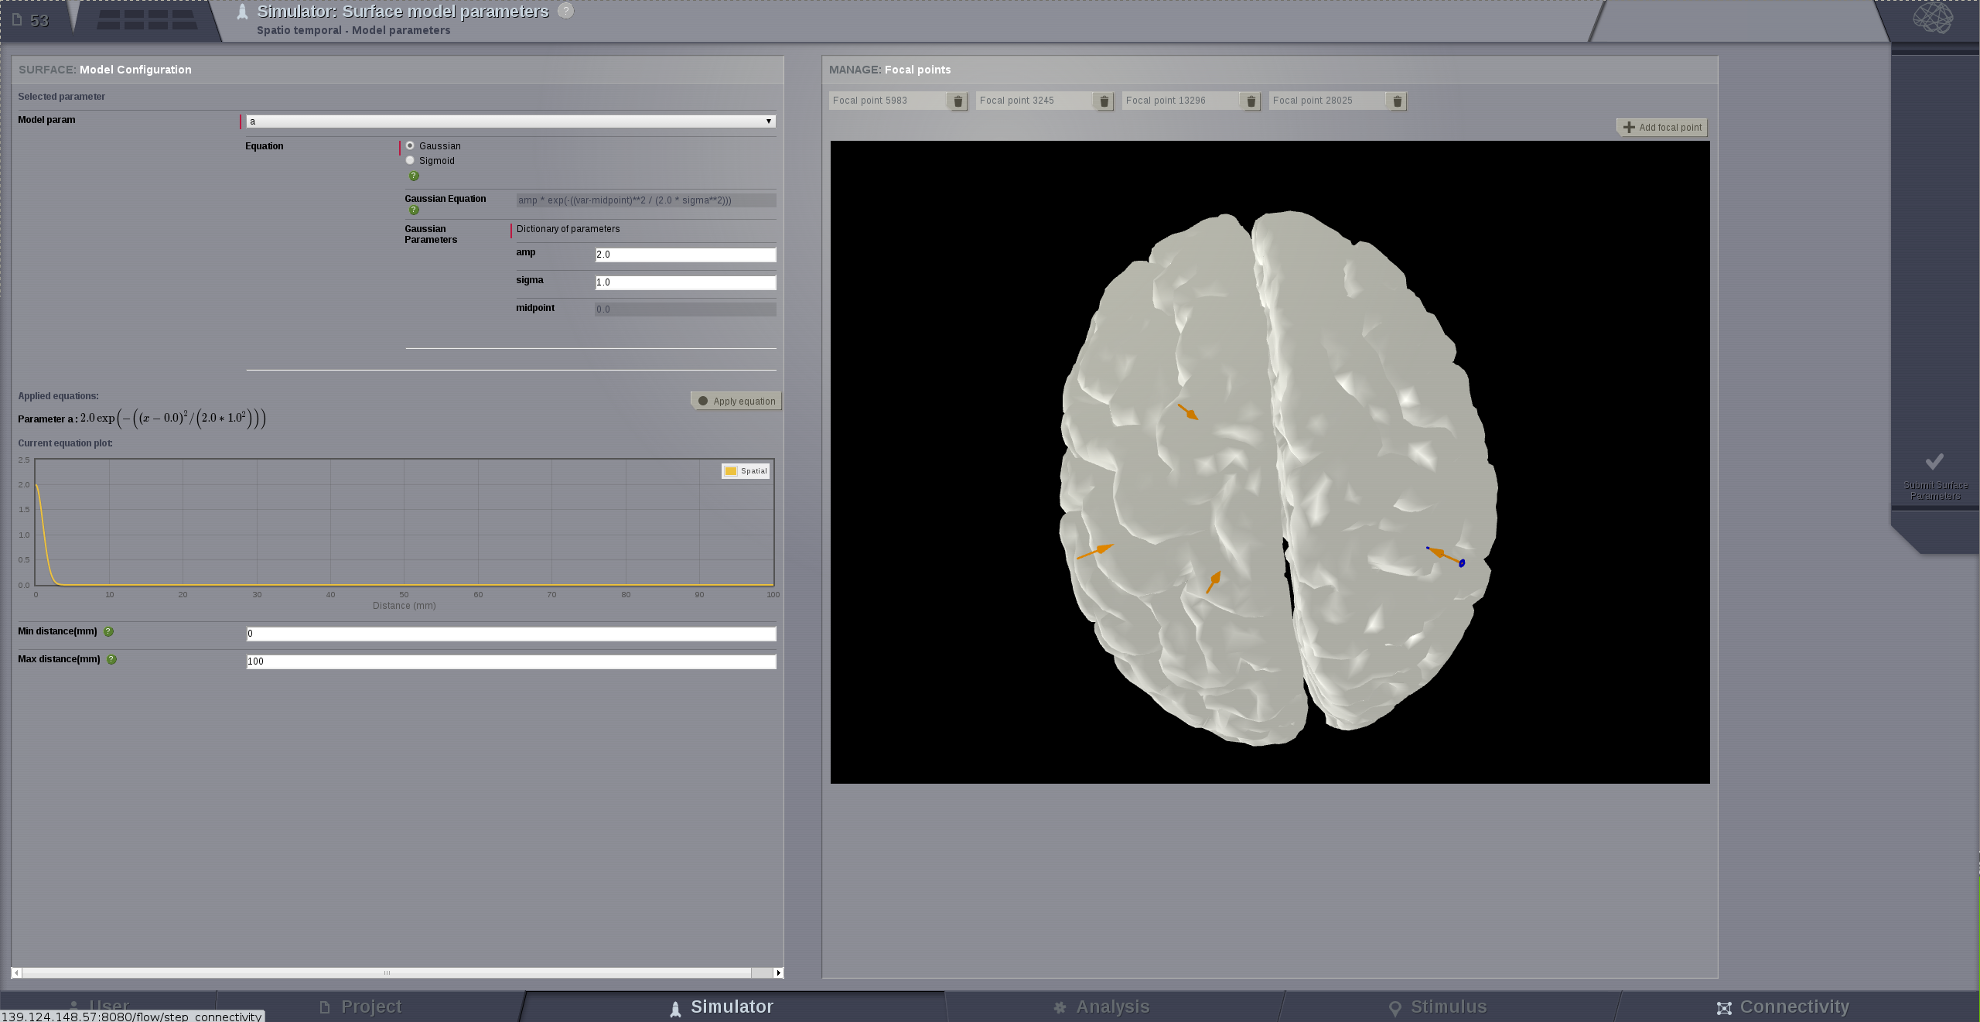
\includegraphics[width=0.47\textwidth]{images/ui_simulator_setup_surface.png}}
			\\
			\subfloat[][]{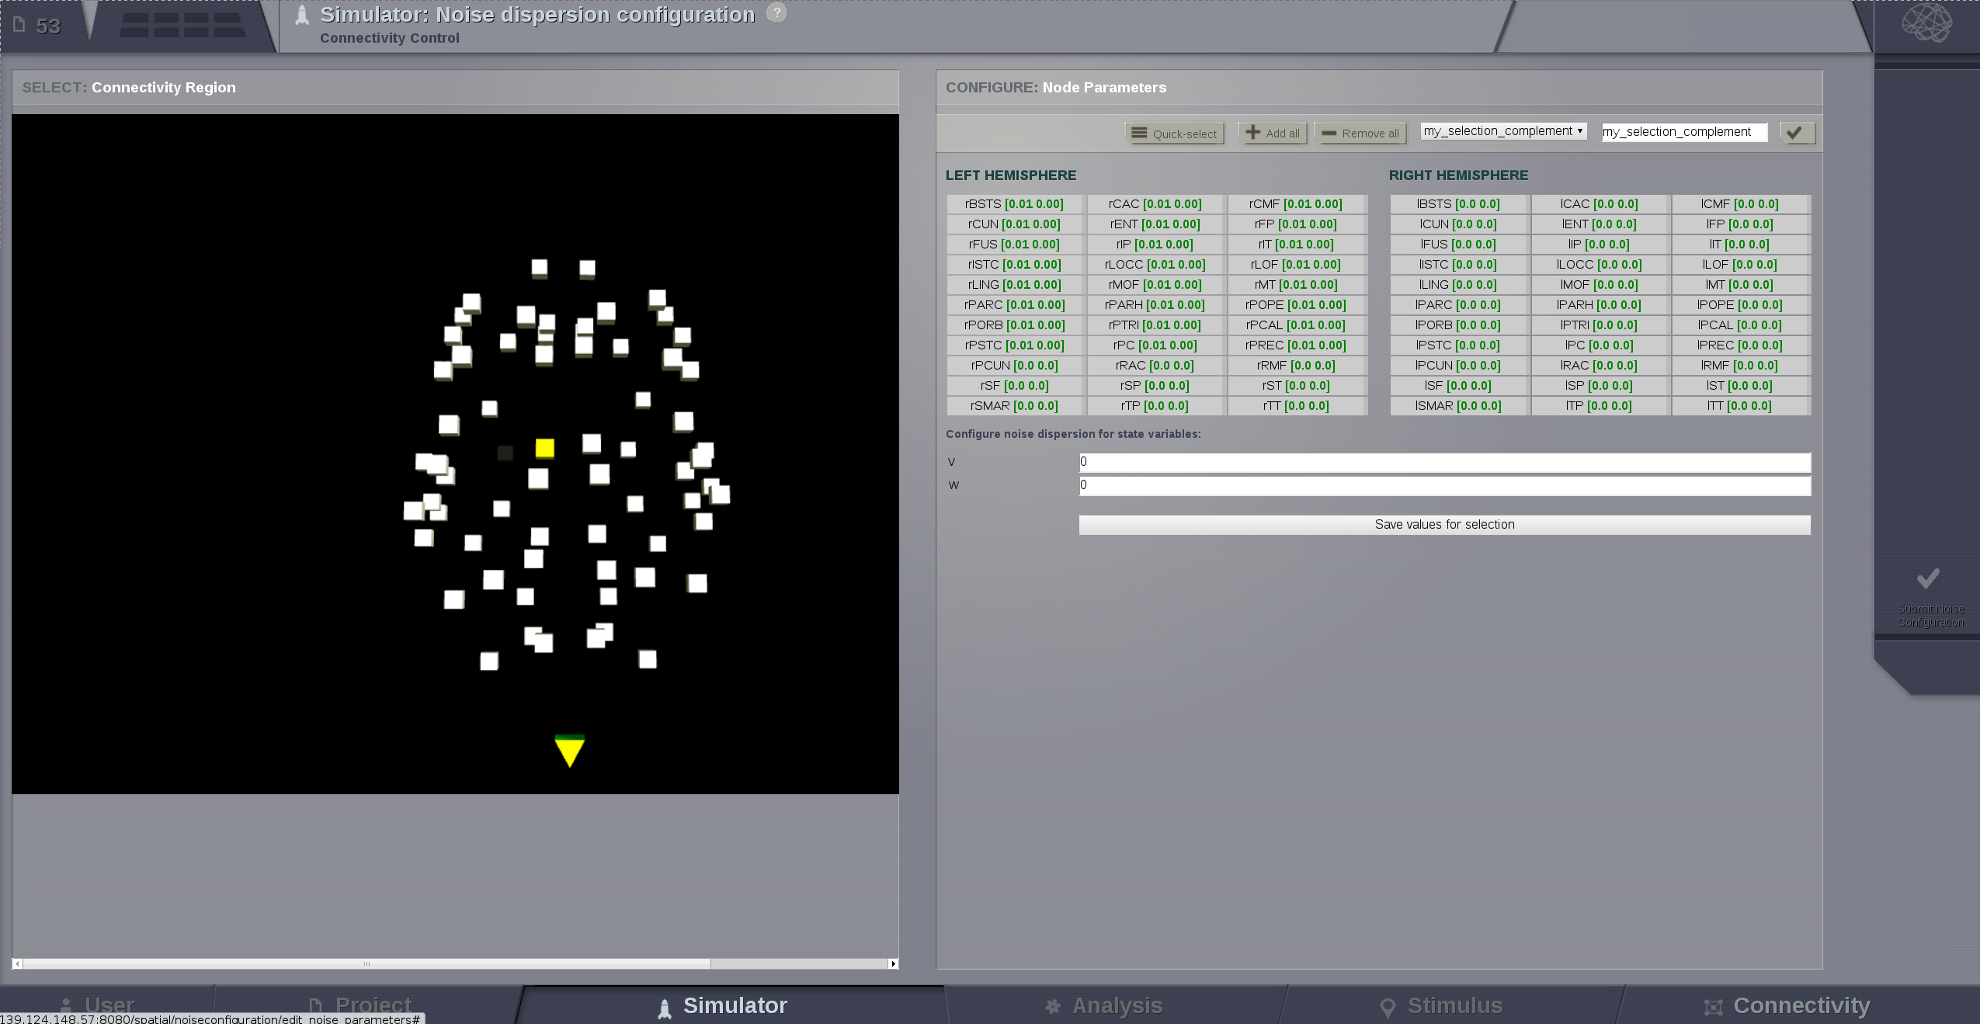
\includegraphics[width=0.47\textwidth]{images/ui_simulator_setup_region_noise.png}}
			\caption{\TVB Simulator Area: 
                (A) View of the main interface. \textit{Left}, the history column displays the
                information about the simulations and their status; \textit{middle}, the
            simulation column is where simulations are configured,
            change of model, parameters, simulation length; \textit{right}, the
            visualization column, provided configurable, multipanel
            visualizers to display the resulting time series or other visualizers
            that will add an analysis step before displaying the results.  (B)
            Region-based simulation configuration. The parameters of the
            mass model can be set independently for each node.  (C) Surface-based
            simulation configuration, allowing the user to define spatially
            inhomogeneous parameters. (D) Define parameters of the simulation's noise. }
		\label{fig:simulator}
		\end{figure}

		The \emph{Simulator} page is a configurable multicolumn interface 
        that combines TVB simulation, analysis and visualization functionalities (Fig.\ref{fig:simulator} A).

		In the left column, a history of all simulations is kept, allowing
        quick access to previous results and their metadata. Here, the user
        may check metadata, add tags and rename or delete the simulation.

		The middle column of the \emph{Simulator} area is where users configure their
		large-scale brain network model. On the top of this column there is a blank
		field to name each particular configuration and a button to launch simulations.
		Via this column, users have access to all the configurable components that might
		be used in a simulation, namely:

		{\small

		\begin{itemize}
			\item long range connectivity (i.e., the connectome or connectivity matrix);
			\item long range coupling function (to scale the weights in the connectivity matrix);
			\item conduction speed;
			\item cortical surface;
			\begin{itemize}
				\item local connectivity kernel;
				\item local connectivity strength (can be configured to be different for each vertex);
				\item region mapping (correspondences between vertices of the surface and anatomical regions in the connectome);
			\end{itemize}
			\item stimulus
			\item local dynamics model (i.e. neural mass model)
				\begin{itemize}
					\item state variable range;
					\item state variables to be recorded and stored;
					\item initial conditions (seed and type of noise used to set random initial conditions);
				\end{itemize}
			\item integration scheme;
			\begin{itemize}
				\item if stochastic, the random seed can be set as well as the type of noise (white, coloured);
				\item integration time step size;
			\item monitors (you can set the monitors period to downsample the raw time-series)
			\item simulation length
			\end{itemize}
		\end{itemize}
		}

		Additional information about the components (e.g., modules, datatypes
		and their attributes) is available  by clicking on the question
		mark icon next to each element. This documentation is pulled from the
		annotations provided by the traits system and documentation strings.

		Specific pages are accessible for setting up the neural mass model
		parameters in region-based and surface-based simulations, as well as
		for configuring the noise amplitude in stochastic integrations (only
		for region-based simulations) (Figs. \ref{fig:simulator} B, C and D)
		The ``Set up region Model'' area consist of an interactive phase-plane
		display. This tool shows the 2-dimensional planes of the general
		N-dimensional phase space of the local dynamic model. This tool is
		used to observe how the dynamics of the physical model change as a
		function of its parameters, acting as a guide to set those parameters
		appropriately.

		On the right column, different displays can be configured to show 
		the simulated time series and to add an analysis step with a subsequent
        visualization of the
		results, for example, computing the correlation coefficients and visualizing the
		resulting matrix.

        For many of the parameters, such as 
        a parameter of the local dynamics model, coupling
		strength, conduction speed, among others, 
        it is possible to specify a range of evenly
        spaced values, and launch the corresponding sweep in
        parallel, using several CPU cores. When the simulation results
        are available, a common metric, such as average variance or 
        degree of synchronization, is applied to the time series, and a 
        one or two dimensional plot, determined by the number of parameters
        for which parameter ranges were provided, is shown, allowing
        the user to see how the simulation changes with the chosen parameters
		(Fig.\ref{fig:visualizers} D).
		
		\subsubsection{Analysis \& Visualizers}

			TVB does not intend to provide fully featured, complex data analysis
            techniques, which have been well covered by other packages. 
            Instead, we offer a minimal set of standard algorithms to quickly
            validate simulation results or compare with imported patient data; 
            these include principal and independent component analyses, 
            Fourier and wavelet spectral analyses, correlation and coherence
            analyses, and for connectivity, an interface to the Brain 
            Connectivity Toolbox \citep{Rubinov_2010}. 

			For each of the datatypes produced in TVB, one or more
			visualizers are available, each taking advantage of the best
            techniques available:

			 \begin{figure}[!htbp]
					\subfloat[][]{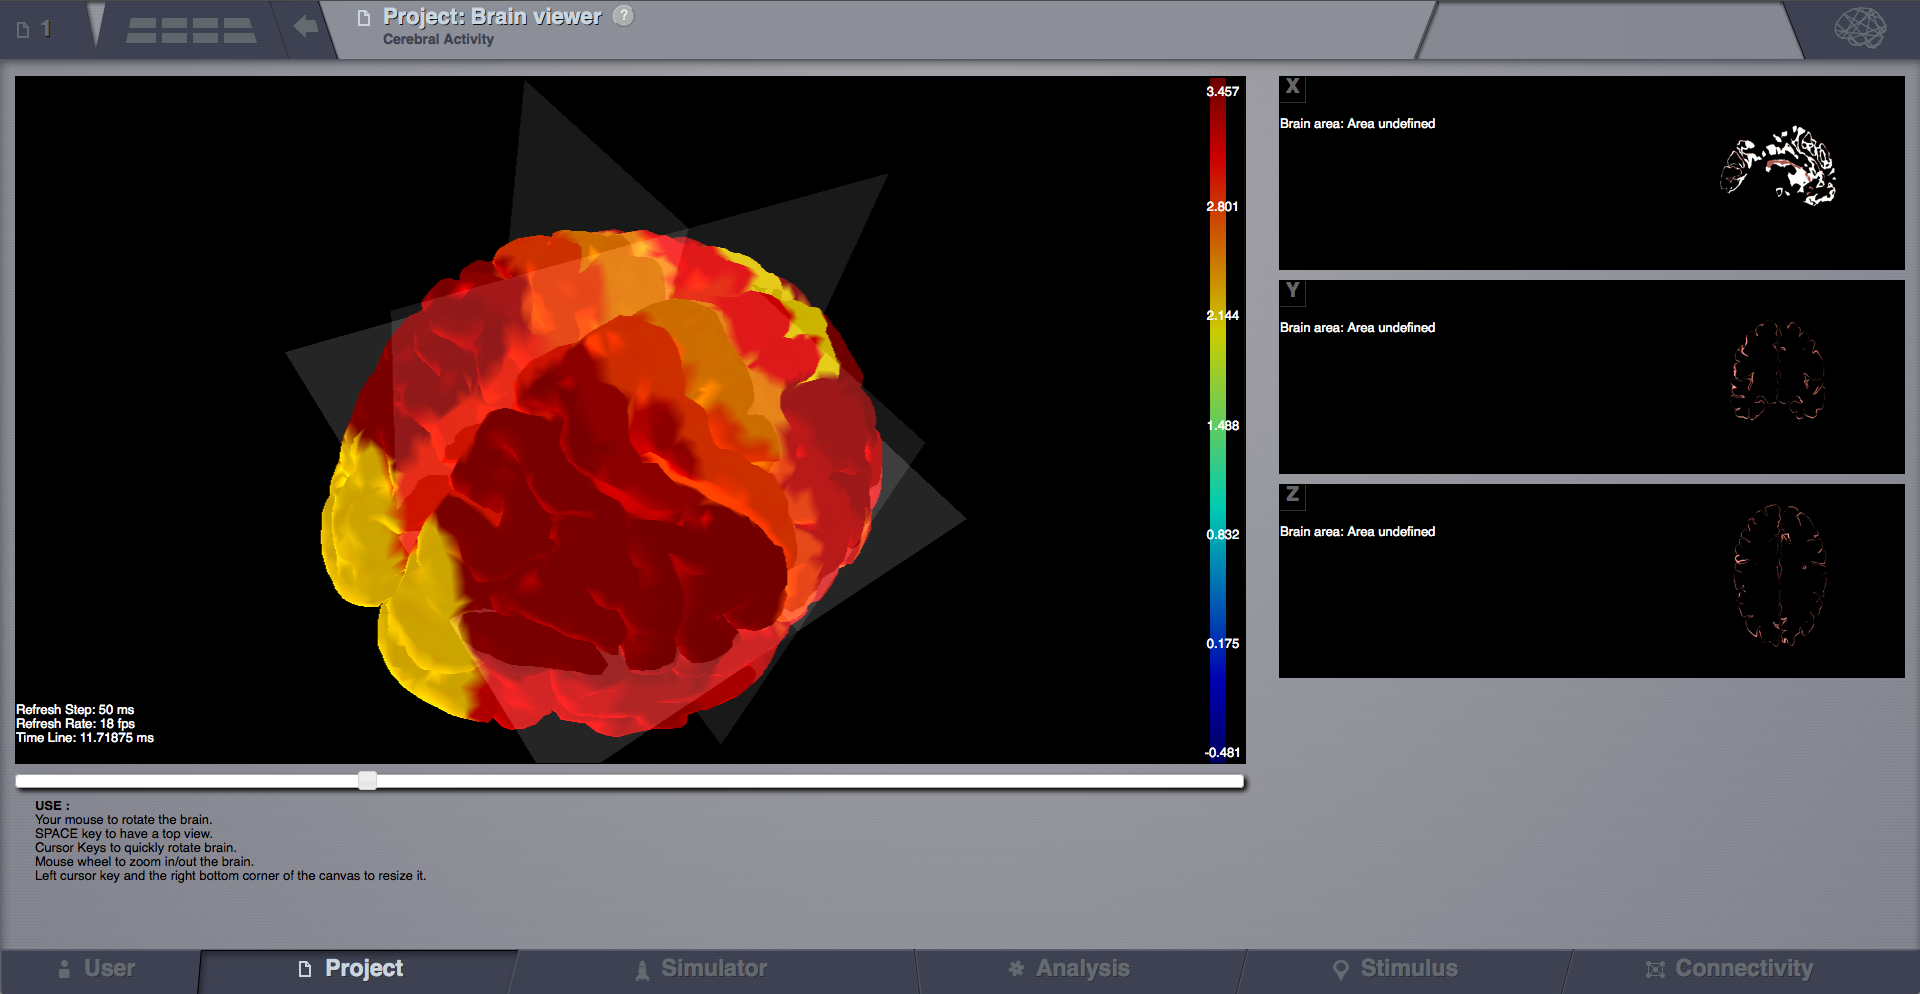
\includegraphics[width=0.48\textwidth]{images/ui_view_brain.png}}
					\\
					\subfloat[][]{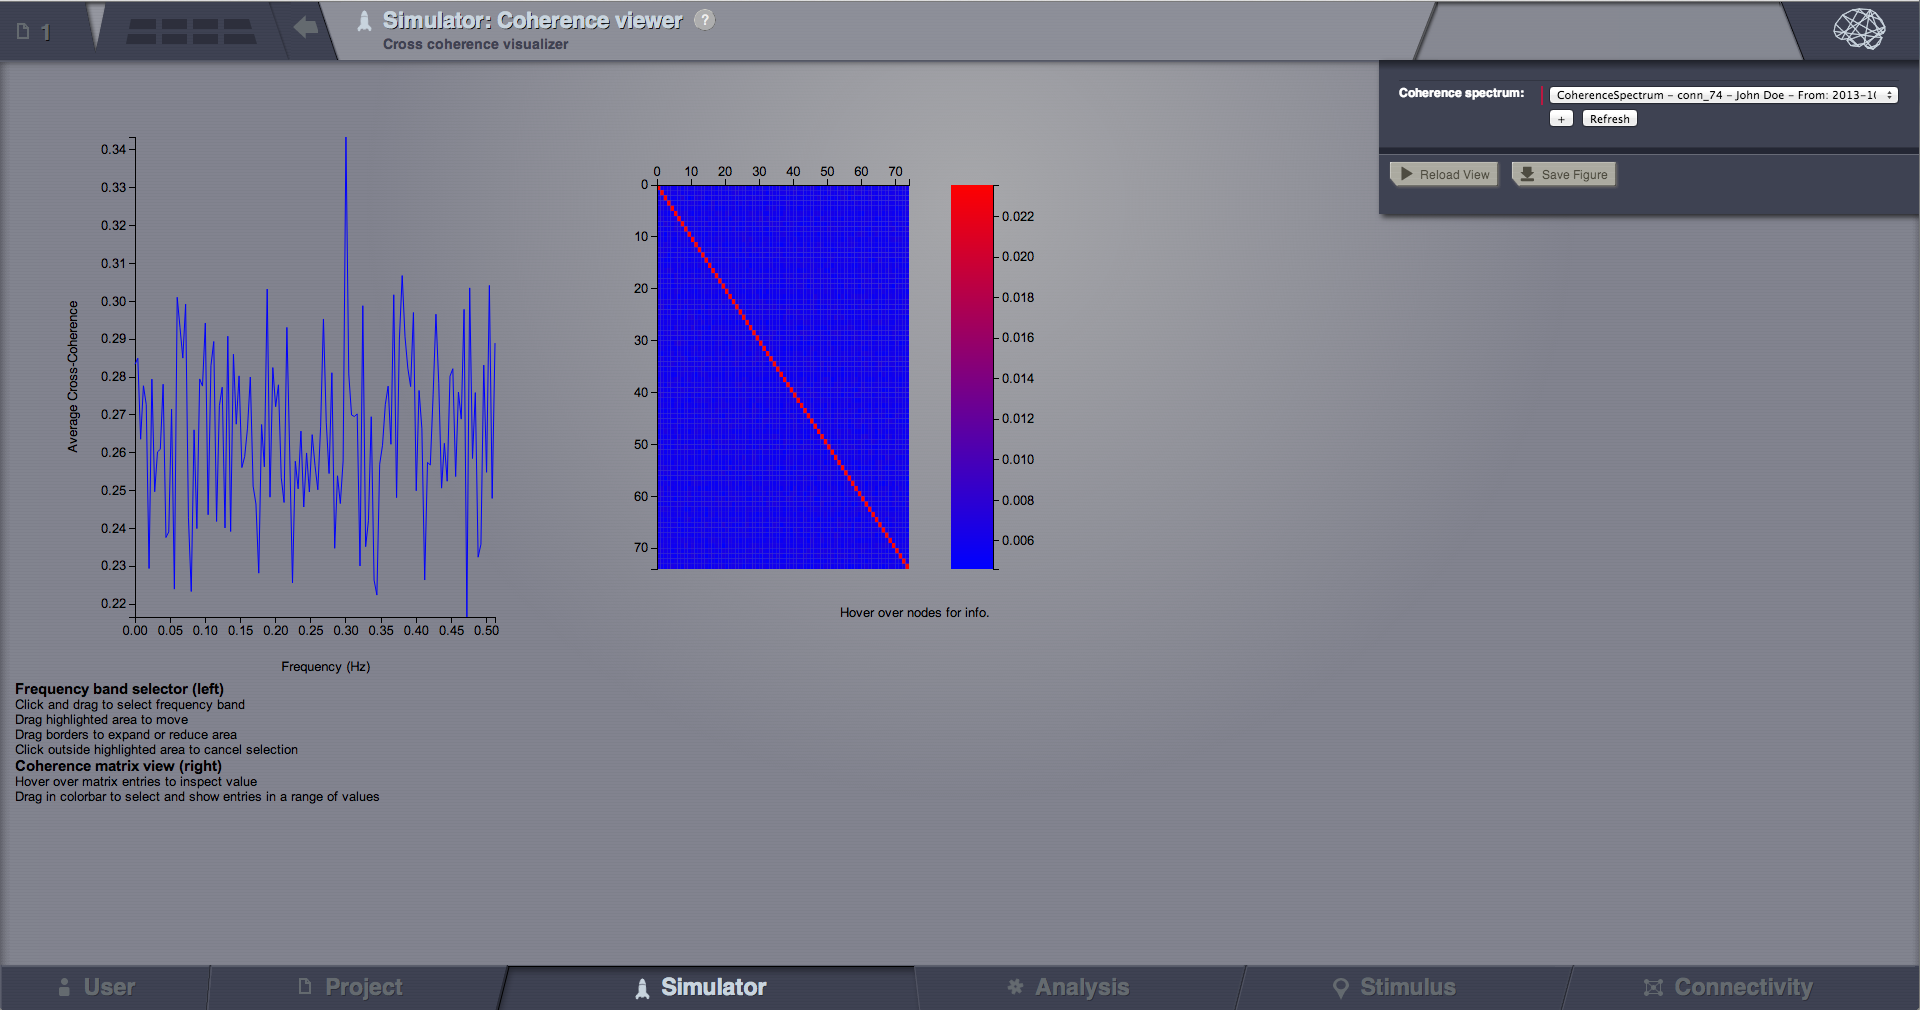
\includegraphics[width=0.48\textwidth]{images/ui_view_coherence.png}}
					\\
					\subfloat[][]{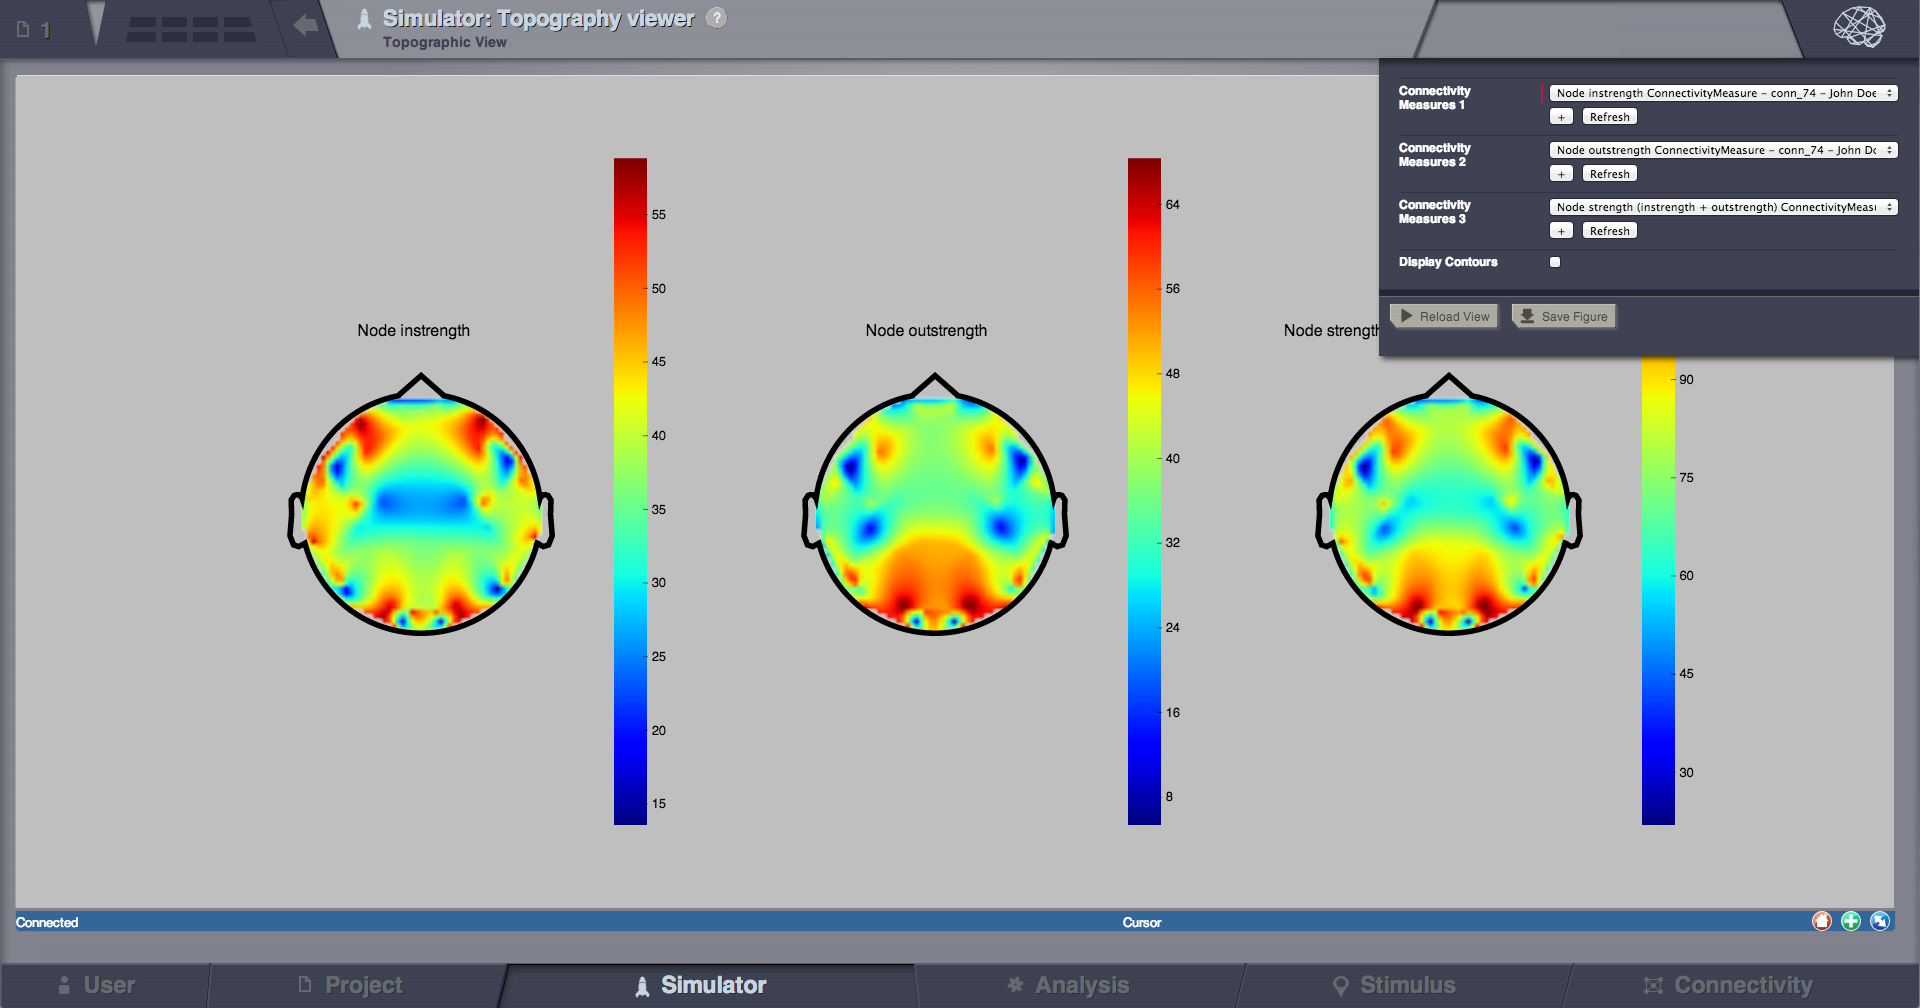
\includegraphics[width=0.48\textwidth]{images/ui_view_topo.png}}
					\\
					\subfloat[][]{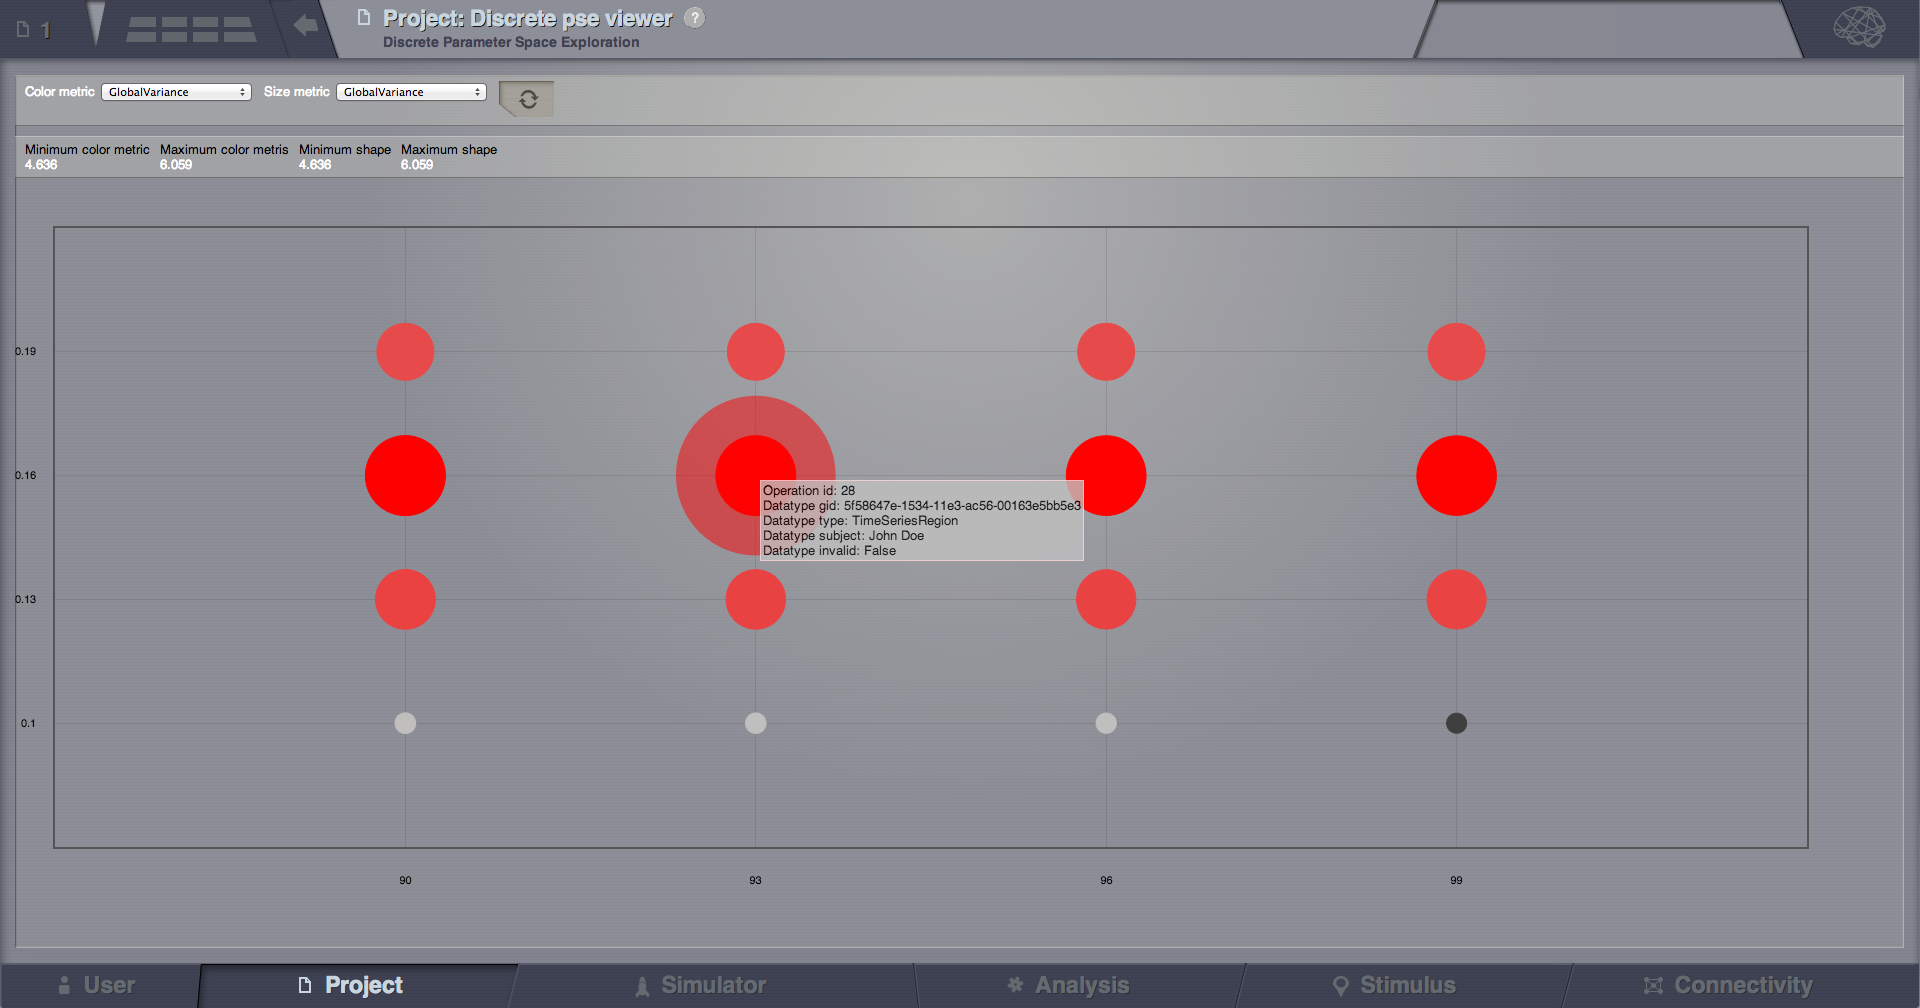
\includegraphics[width=0.48\textwidth]{images/ui_view_pse.png}}
					\caption{\TVB visualizers: 
					(A) WebGL: 3D display of region level simulated signal, mapped on a brain cortical surface
					(B) SVG: Cross Coherence
					(C) MPLH5:  Topographic view with Connectivity in/out strength measures
					(D) FLOT: Parameter Space Exploration results grid}
				\label{fig:visualizers}
			\end{figure}
	
	\begin{enumerate}
		\item \emph{WebGL viewers} are based on \emph{HTML 5 Canvas} element
		and the \emph{GL} context. These viewers offer a 3D display,
		 user interaction with the scene (rotate,
		translate, zoom), and high performance for complex visualizations.
        WebGL is used primarily for visualizing cortical surfaces.
		
		\item \emph{SVG viewers} use a high-quality, highly interactive vectorial 
            format. We
		use such viewers for manipulating and displaying time series,
		covariance or cross coherence datatype results. These visualizers
		were developed specifically for these data types in TVB, and provide a 
		richer level of interaction.

		\item \emph{MPLH5 viewers} use  emph{Matplotlib}'s \emph{HTML 5}
		backend for viewing some of TVB's datatypes, such as
		the Fourier and spectral analyses. 

		\item \emph{Other} simpler viewers in TVB use the JIT
		\url{http://philogb.github.io/jit/} or FLOT
		\url{http://www.flotcharts.org/} Javascript libraries. These are mainly
		2D plots for simple TVB generated data.
	\end{enumerate}

\subsubsection{Connectivity Tools}

		\emph{Connectivity}, in the context of TVB, is another datatype, mapping structural
		information about a subject (a real single individual or an average template). For
		editing and viewing a connectivity, TVB has a dedicated interface, where
		the \emph{G-User} can manipulate connectivity strength and lengths
		at the granularity of individual edges.
        Note that we do not store or use information about the exact trajectory of
		a connection, only the region centers and connection weights and
		lengths.

 \begin{figure}[!htbp]
		\centering
		\subfloat[][]{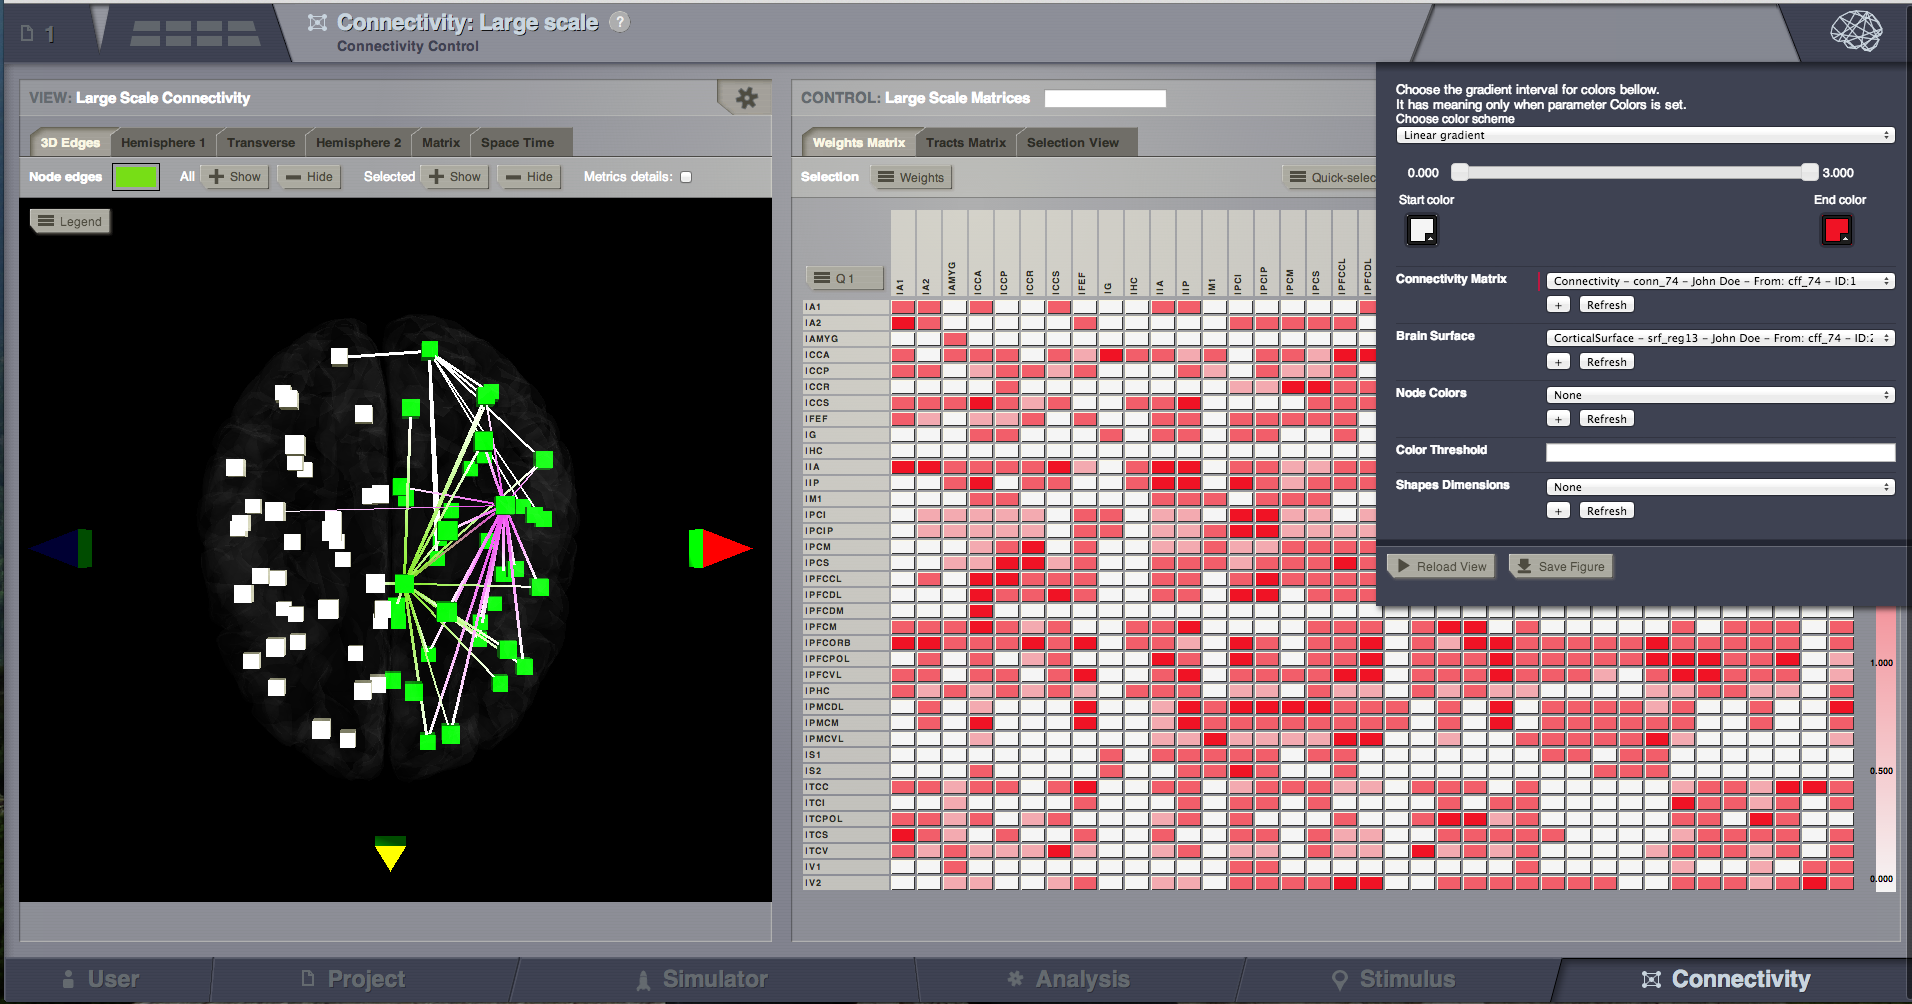
\includegraphics[width=0.48\textwidth]{images/ui_connectivity.png}}
		\\
		\subfloat[][]{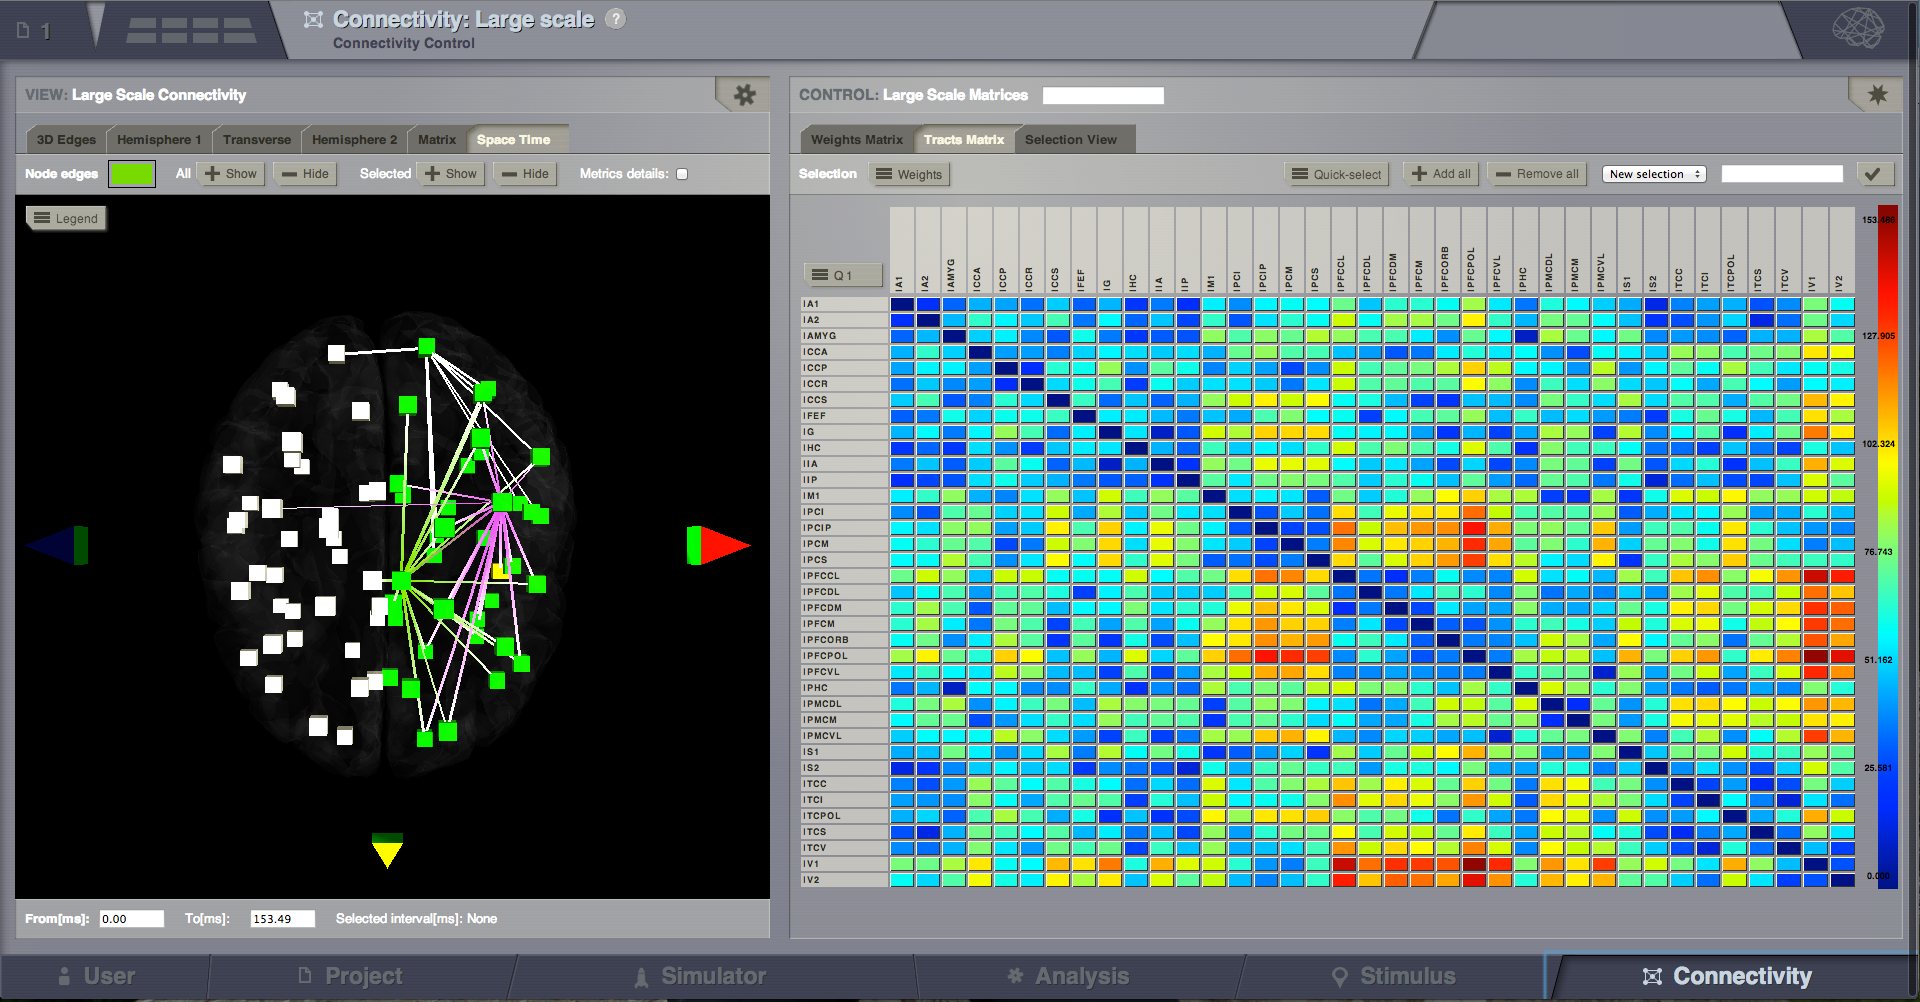
\includegraphics[width=0.48\textwidth]{images/ui_connectivity_delays.png}}
		\caption{Connectivity tools: 
            (A) \textit{Left}: Displaying weighted connections between selection of nodes, with 3D manipulation.
            \textit{Right}: Editing weight connections, one at a time, or many.
            (B) \textit{Left}: Show effect of connectivity delays (in milliseconds) when conduction speed is 1 mm/ms.
        \textit{Right}: Editing and displaying one quadrant from the matrix of connection tracts.}
				\label{fig:connectivity}
\end{figure}

\subsubsection{Stimulus Editor}

    The \emph{Stimulus} interface assists users in generating
	stimulation patterns that may be used later in a simulation, for 
    example to model the effects of transcranial magnetic stimulation.
    The way in which stimuli are designed depends on whether the simulation
    will be at region-based or surface-based.
	For region-based simulations, a
	unique temporal profile can be specified for each node, with the amplitude
	of the stimulation modulated individually for each node. For surfaces,
	in addition to the temporal profile, it is possible to select several vertices
	on the surface to define the foci around which the spatial pattern is centered.
    A stimulation profile in TVB is a \emph{pattern}
	datatype, either uniquely temporal or spatiotemporal depending the
	spatial support of the network.

\subsection{Console and scripting}

The components of TVB are of course accessible from a Python
script or, more conveniently, from any of the IPython interfaces.
For example, the tutorials for the simulator have been developed
as IPython notebooks, due to its ability to mix text, mathematics,
code and figures. 

\subsubsection{\texttt{hello\_brain.py}}

To give a basic feel for scripting TVB simulations, we will 
walk through a simple example of a region-level simulation.

\begin{lstlisting}
from tvb.simulator.lab import *
\end{lstlisting}

\noindent which is an all-in-one module making writing scripts
shorter, in the style of \texttt{pylab}, as it imports everything
from \texttt{pylab}, \texttt{numpy} and most of TVB's simulator
modules. Next, we build a simulator object:

\begin{lstlisting}
sim = simulator.Simulator(
    model        = models.Generic2dOscillator(), 
    connectivity = connectivity.Connectivity(),
    coupling     = coupling.Linear(a=1e-2),
    integrator   = integrators.HeunDeterministic(),
    monitors     = (
            monitors.TemporalAverage(), 
    )
)
\end{lstlisting}

\noindent where we've employed a two dimensional oscillator
with default parameters, the default connectivity, a linear 
coupling function with a slope of $1e-2$, and deterministic
Heun integrator and a monitor that temporally averages the 
network dynamics before providing output. Each of these
components can be replaced by a user's subclass of the
appropriate base class, e.g. the value of \texttt{model}
should subclass \texttt{models.Model}.

While TVB strives to keep modules independent of one another,
it is typical for mathematical dependencies to arise between, 
for example, the mass model and the integration time step, so
after configuring a simulator object, it is necessary to invoke

\begin{lstlisting}
sim.configure()
\end{lstlisting}

\noindent which results in walking the tree of objects, checking and 
configuring the constraints among parameters recursively.

The next step is to run through the simulation, collecting
output from the simulator. In this case, it is as simple as

\begin{lstlisting}
ys = array([y for ((t, y),) in  sim(simulation_length=3e2)])
\end{lstlisting}

\noindent where the simulator has been called, returning a 
generator which performs the integration and returns, for each
monitor, the current time and activity. In a case where EEG 
and fMRI monitors, for example, were used, we might write

\begin{lstlisting}
eeg, mri = [], []
for (t_eeg, y_eeg), (t_mri, y_mri) in sim(3e2):
		if y_eeg is not None:
		eeg.append(y_eeg)
		...
\end{lstlisting}

\noindent Because fMRI and EEG monitors have very different
timescales, whenever one monitor return data and the others do
not, the others contain \texttt{None}, hence the check. Building
more complex logic in this loop would permit, for example, online
feedback and modification of connectivity. 

After the simulation loop has finished, you may wish to see the
result, following the previous listing, 

\begin{lstlisting}
plot(ys[:, 0, :, 0], 'k', alpha=0.1)
\end{lstlisting}

\noindent Here we note that \texttt{ys} is four dimensional. The 
simulator has the convention of treating  mass model state as a
three dimensional array of state variables by nodes by statistical
modes. Because \texttt{ys} is an array collected over time, the first
dimension is time, and the plot here is of each node's first state
variable, over time.

Many more demonstrations of the various features of the simulator
can been found in scripts distributed with the sources of TVB, or 
browsed online at \url{https://github.com/the-virtual-brain/scientific_library/tree/trunk/tvb/simulator/demos}.

For more details see the IPython notebook Tutorial: Anatomy of a Region Simulation 
\url{http://nbviewer.ipython.org/urls/raw.github.com/the-virtual-brain
/scientific_library/trunk/tvb/simulator/doc/tutorials/Tutorial_Anatomy
_Of_A_Region_Simulation/Tutorial_Anatomy_Of_A_Region_Simulation.ipynb}

\section{Conclusions}

Since the recent release of the $1.0$ version of TVB, it has been 
officially considered \textit{feature} complete, however, in several
cases, the development of features has outstripped documentation 
and testing. Going forward, general priorities include
advancing test coverage, improving documentation for users, and
preparing PyPI and Debian packages. In the mean
time, TVB's Google groups mailing list continues to
provide an open forum for troubleshooting and sharing of user experiences.

The literature on network models frequently presents work in which a model
is constructed in order to estimate structure and parameters from 
experimental data, and the DCM framework has significantly advanced 
methods for such estimations for both fMRI and M/EEG data. Indeed, there
are similarities in the underlying mathematical machinery between DCM and 
TVB. However, the estimation of parameters in the case of TVB's models
is still a challenging question and for now is not a goal of the framework. 
For this reason, none of the requisite estimation tools are currently 
provided by TVB.

Related to the goal of estimating model parameters for brain network models
is the modeling of function or functional dynamics itself 
\citep{erlhagen2002dynamic, eliasmith2012large}. TVB allows a user
to fully specify the node dynamics and connectivity, yet no support
is currently providing for deriving a set of parameters that leads to 
a particular functional state. This, like the estimation problem, is 
an open question, particularly for models as complex as those simulated 
within TVB.

While several mathematical challenges are presented by the TVB models, 
one of the bottlenecks is the speed of the numerical simulation.
To address this, continued optimization of C and GPU code generation
will take place, e.g. to perform parallel parameter sweeps. 

Additionally, an interface \textit{from} MATLAB to TVB 
is being developed to allow use of the simulator through a simple
set of MATLAB functions. As this infrastructure is based on an HTTP and 
JSON API, it will likely enable other applications to work with TVB as well.

Lastly, as TVB was originally motivated to allow a user to move from acquired
data to simulated data as easily as possible, we will continue to integrate
several of the requisite steps that are not currently covered, such as analysis
of DSI data to produce connectivity matrices, though in many cases, such as
parcellation and labeling of cortical areas, these steps may continue to
require intervention with other software. Nevertheless, TVB provides a
promising platform for integrating neuroinformatics tools with an emphasis on
analysis and modeling of human neuroimaging data.

%\begin{enumerate}
%	\item Diffusion tensor imaging \& tractography pipeline to convert
%        MRI data into connectivity data.
%	\item Connectome project on structural connectivity
%	\item Structural imaging processing via FreeSurfer (pySurfer, NiPy, etc.)
%	\item NeuroML model specification 
%\end{enumerate}


\section*{Acknowledgments}
Several authors have also participated in the
development of TVB. They are listed in the \texttt{AUTHORS} file 
of the source code and deserve our warm acknowlegments. LP wishes to thank
specifically Y.~Mahnoun for his role in the design and development
of the first prototype of the TVB architecture. The research reported herein
was supported by the  Brain Network Recovery Group through the James S.
McDonnell Foundation and the FP7-ICT BrainScales. PSL and MMW received
support by from the French Minist\`{e}re de Recherche and the Fondation
de Recherche Medicale.

\bibliographystyle{apalike}
\bibliography{bib}

\end{document}

